\chapter{Livello applicazione}

\section{Introduzione}
Il livello applicazione fornisce servizi all'utente. La comunicazione è fornita per mezzo di una connessione logica: questo significa che i livelli applicazione nei due lati della comunicazione agiscono come se esistesse un collegamento diretto (immaginario) attraverso il quale poter inviare e ricevere messaggi.

\begin{Example}{Connessione logica a livello applicazione}{}

    \begin{minipage}[c]{0.53\textwidth}
        La figura illustra uno scenario nel quale un ricercatore che lavora nell'azienda Sky Research deve ordinare un libro relativo alle proprie ricerche dalla libreria online Scientific Books. La connessione logica avviene tra il livello applicazione di un client in Sky Research e il livello applicazione di un server nella libreria. I due utenti (Gaia e Gabriele) possono immaginare che tra di essi esista un canale logico bidirezionale, attraverso il quale si possono inviare dei messaggi. La comunicazione reale, tuttavia, avviene attraverso più dispositivi (Gaia, R2, R4, R5, R7 e Gabriele) e vari canali fisici.
    \end{minipage}
    \hfill
    \begin{minipage}[c]{0.45\textwidth}
        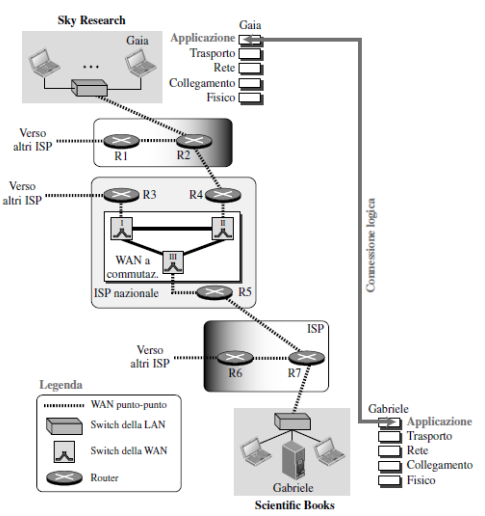
\includegraphics[width=1\textwidth]{images/liv-applicazione.PNG}
    \end{minipage}
\end{Example}

\subsection{L'offerta dei servizi}
Tutte le reti di comunicazione sviluppate prima di Internet avevano l'obiettivo di fornire servizi ai propri utenti; la maggior parte di queste reti, tuttavia, era inizialmente progettata per offrire un servizio specifico.

Anche Internet venne originalmente progettata con lo stesso scopo: fornire servizi agli utenti in tutto il mondo. Un nuovo protocollo che viene aggiunto ad un dato livello deve essere progettato in modo tale da utilizzare i servizi offerti da uno dei protocolli di livello inferiore. Se un protocollo viene eliminato da un livello, è necessario apportare le modifiche necessarie ai protocolli del livello immediatamente superiore, che utilizzavano i servizi del protocollo rimosso.

Il livello applicazione, tuttavia, ha caratteristiche peculiari rispetto agli altri protocolli della pila, visto che si trova nel livello più alto. I protocolli di questo livello non forniscono servizi ad altri protocolli di livello superiore, ma utilizzano solamente i servizi offerti dai protocolli del livello inferiore (quello di trasporto). Questo significa che eliminare protocolli da questo livello è un'operazione facile, cosi come aggiungere nuovi protocolli purché questi siano in grado di utilizzare i servizi di uno dei protocolli di livello trasporto.

Dato che il livello applicazione è l'unico che fornisce servizi agli utenti di Internet, la sua flessibilità consente di aggiungere nuovi protocolli con estrema facilità.

\subsubsection*{Protocolli standard e non standard}

Per agevolare le operazioni di Internet, i protocolli utilizzati nei primi quattro livelli dello stack TCP/IP devono essere standardizzati e opportunamente documentati. Per una maggiore flessibilità, tuttavia, i protocolli di livello applicazione possono essere sia standard che non standard.

\begin{itemize}
    \item Esistono diversi protocolli di livello applicazione che sono stati standardizzati e documentati dagli enti responsabili della gestione di Internet. Ogni protocollo standard è costituito da una coppia di programmi che interagiscono con l'utente e con il livello trasporto per fornire un servizio specifico.
    \item E' possibile creare un'applicazione non standard scrivendo due programmi che forniscono servizi agli utenti, facendo uso dei servizi di trasporto. La possibilità di creare protocolli non standard che non richiedono alcuna approvazione: un'azienda privata può sviluppare il proprio protocollo specifico di livello applicazione per comunicare con i propri uffici sparsi nel mondo, utilizzando i servizi offerti dai primi quattro livelli dello stack TCP/ IP, senza essere costretta ad utilizzare alcun programma applicativo standard.
\end{itemize}

\subsection{Paradigmi del livello applicazione}
Dovrebbe ormai essere chiaro che per utilizzare Internet sono necessari due programmi che interagiscono l'uno con l'altro: uno eseguito su un certo computer in qualche parte del mondo, l'altro eseguito su un secondo computer in qualsiasi altro luogo. I due programmi hanno la necessità di scambiarsi messaggi sfruttando l'infrastruttura di Internet. I due programmi applicativi devono essere entrambi in grado di richiedere e offrire servizi, oppure ciascuno deve occuparsi di uno dei due compiti? Con il passare del tempo, sono stati sviluppati due approcci (paradigmi) diversi: il paradigma client/server e quello peer-to-peer.

\subsubsection*{Paradigma client/server}
L'approccio tradizionale è chiamato client/server, ed è stato il paradigma più utilizzato fino a pochi anni fa. Con questo paradigma il fornitore di servizi è un programma applicativo chiamato processo server, sempre in esecuzione in attesa che un altro programma applicativo, chiamato processo client, apra una connessione via Internet e richieda un servizio. Vi sono solitamente un numero limitato di processi server pronti ad offrire uno specifico servizio, ma numerosi client che richiedono servizi da questi server. Il processo server deve essere in esecuzione permanente, il processo client viene mandato in esecuzione solo quando ha bisogno di ottenere un servizio.

Sebbene la comunicazione nel paradigma client/server avvenga fra due programmi applicativi, il ruolo di ciascun programma è totalmente differente. Infatti non è possibile eseguire un client come programma server e viceversa.

\begin{figure}[ht]
    \centering
    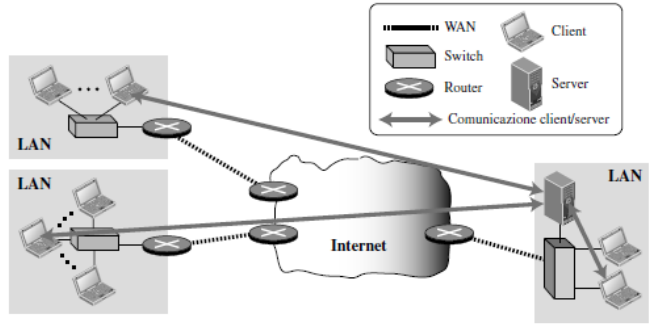
\includegraphics[width=9cm]{images/client-server.PNG}
    \caption{Esempio di architettura client/server}
    \label{fig:client-server}
\end{figure}

Un problema di questo paradigma è che il carico di comunicazione risulta concentrato sul server, che deve quindi utilizzare un computer con molte risorse di comunicazione e computazione. Un secondo problema è che deve esservi un fornitore di servizi disponibile a sobbarcarsi il costo della complessa infrastruttura necessaria per offrire un particolare servizio. Affinché questo possa avvenire, il servizio dovrà quindi necessariamente fornire un qualche tipo di ritorno economico.

Numerosi servizi tradizionali utilizzano ancora questo paradigma, tra cui il World Wide Web (WWW) con il protocollo associato HTTP (HyperText Transfer Protocol), il File Transfer Protocol (FTP), il protocollo Secure Shell (SSH), la posta elettronica e così via.

\section{WEB e HTTP}
Fino agli anni '90 Internet veniva principalmente utilizzata da ricercatori, docenti e studenti universitari per raggiungere host remoti, trasferire file, ricevere e inviare notizie e per la posta elettronica. Poi, nei primi anni '90, comparve sulla scena una nuova importante applicazione: il World Wide Web. Il Web è stata la prima applicazione Internet che ha catturato l'attenzione del pubblico, cambiando profondamente il modo di interagire all'interno e all'esterno degli ambienti di lavoro. Forse ciò che attira di più gli utenti è che il Web opera su richiesta (on demand): si può avere ciò che si vuole, quando lo si vuole. Inoltre, è facilissimo per tutti rendere disponibili informazioni sul Web: chiunque può diventare editore a costi estremamente bassi e i collegamenti ipertestuali e i motori di ricerca ci aiutano a navigare in un oceano di siti.

\subsection{Panoramica Web}
\subsubsection*{Architettura}
Il Web è oggi un servizio client/server distribuito, nel quale un client che utilizza un browser può accedere a un servizio offerto da un server. Il servizio fornito è tuttavia distribuito su numerose locazioni fisiche chiamate siti. Ogni sito contiene uno o più documenti chiamati pagine web, ciascuna delle quali può contenere collegamenti (o riferimenti) ad altre pagine web nello stesso sito o in altri siti.

\begin{Example}{Architettura Web}{}
    \textit{Si supponga di voler ottenere un documento scientifico che contiene un riferimento a un altro documento testuale e un riferimento a un'immagine.}

    \begin{minipage}{\textwidth}
        \centering
        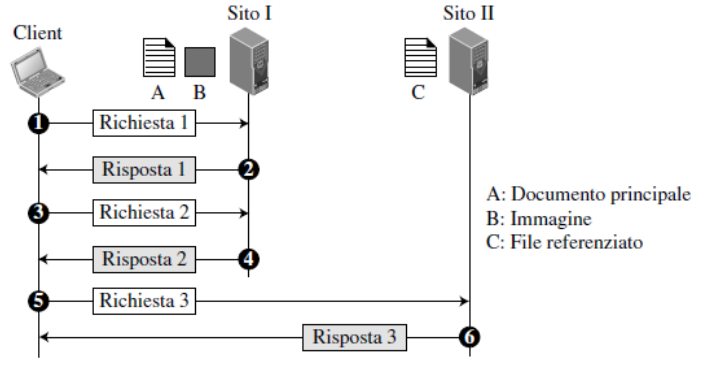
\includegraphics[width=0.6\linewidth]{images/architettura-web.PNG}
        %\captionof{figure}{Esempio}
    \end{minipage}

    Il documento principale e l'immagine sono memorizzati in due file separati nello stesso sito (file A e file B), mentre il documento testuale referenziato è memorizzato in un altro file in un altro sito (file C). Poiché si hanno tre file differenti, sono necessarie tre transazioni per poter vedere il documento completo. La prima transazione (richiesta/risposta) consente di ottenere una copia del documento principale (file A), che contiene dei riferimenti (puntatori) agli altri due file. Quando viene ottenuta una copia del documento principale, l'utente può attivare il collegamento all'immagine per innescare la seconda transazione e ottenere una copia dell'immagine (file B). Se l'utente desidera vedere il contenuto del file di testo collegato, può attivarne il collegamento facendo click con il mouse sul relativo link, innescando la terza transazione per ottenere una copia del file C. Si noti che nonostante i file A e B siano memorizzati nello stesso sito, si tratta comunque di file indipendenti con nomi e indirizzi differenti. Sono necessarie due transazioni per poterli ottenere.
\end{Example}

Esistono numerosi browser, capaci di interpretare e visualizzare i documenti Web, che utilizzano sostanzialmente la medesima architettura. Qualsiasi browser è composto solitamente da tre componenti: il controllore, il modulo che implementa il protocollo client e gli interpreti. Il controllore riceve l'input dalla tastiera o dal mouse e sfrutta i protocolli client per accedere al documento. Ottenuto il documento, il controllore utilizza uno degli interpreti per visualizzarlo sullo schermo. Il protocollo client può essere uno dei protocolli che verranno descritti in seguito, come HTTP o FTP. Gli interpreti possono gestire HTML, Java, JavaScript o altro, a seconda del tipo di documento. Internet Explorer, Google Chrome e Mozilla Firefox sono esempi di browser.

\begin{figure}[ht]
    \centering
    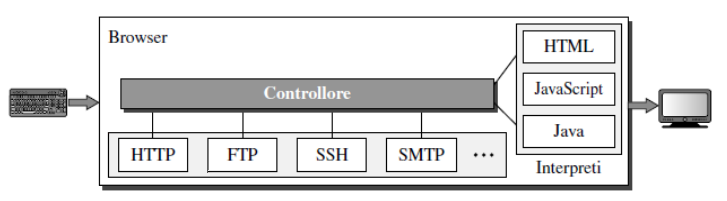
\includegraphics[width=10cm]{images/architettura-browser.PNG}
    \caption{Architettura generale di un browser}
    \label{fig:architettura-browser}
\end{figure}

\subsubsection*{URL (Uniform Resource Locator)}
Una pagina Web, essendo un file, deve avere un identificatore univoco per distinguerla dalle altre pagine. Per identificare una pagina Web sono necessari tre identificatori: host, porta e percorso. Tuttavia, prima di definire la pagina Web è necessario indicare al browser quale applicazione client/server si desidera utilizzare, specificando il cosiddetto protocollo. Per identificare una pagina Web sono quindi necessari quattro parametri: il primo indica lo strumento che deve essere utilizzato per recuperare la pagina Web, la combinazione degli altri tre identifica l'oggetto ricercato (pagina Web).
\begin{itemize}
    \item Il primo identificatore è un'abbreviazione che indica il protocollo client/server necessario per il trasferimento. Nella maggior parte dei casi si tratta di HTTP, ma è possibile utilizzare anche altri protocolli come FTP (File Transfer Protocol).
    \item L'identificatore dell'host può essere l'indirizzo IP o il nome univoco assegnato al server. Gli indirizzi IP possono essere espressi in notazione decimale puntata (per esempio 64.23.56.17). Il nome è solitamente il nome di dominio che identifica univocamente l'host.
    \item La porta, un intero di 16 bit, è predefinito per molte applicazioni client/server standard. Per esempio se si utilizza il protocollo HTTP per accedere alle pagine Web, il numero di porta è 80. E' possibile utilizzare una porta differente, ma in questo caso è necessario indicarne esplicitamente il numero.
    \item Il percorso identifica la posizione e il nome del file nel filesystem. Il formato di questo identificatore dipende normalmente dal sitema operativo utilizzato. In Unix un percorso è una sequenza di nomi di directory seguita dal nome del file, tutti separati da slash (il carattere "/").
\end{itemize}

Questi quattro elementi sono raggruppati assieme sotto forma di URL (Uniform Resource Locator), come ad esempio: \verb|protocol://host/path| è utilizzato nella maggior parte dei casi quando la porta utilizzata è quella standard e \verb|protocol://host:porta/path| è utilizzato quando è necessario specificare il numero di porta.

\subsubsection*{Documenti Web}
I documenti Web possono essere raggruppati in tre categorie: statici, dinamici e attivi.
\begin{itemize}
    \item I documenti statici sono documenti dal contenuto predeterminato che vengono memorizzati in un server. Il client può solamente ottenere una copia di tali documenti. In altri termini, i contenuti sono determinati al momento della loro creazione, non al momento del loro utilizzo.
    \item Un documento dinamico viene creato dal server Web alla ricezione di una richiesta di un browser. All'arrivo della richiesta, il server esegue un programma applicativo o uno script che crea il documento dinamico: il server restituisce al browser l'output del programma o dello script eseguito. Dato che viene creato un nuovo documento per ogni richiesta, il suo contenuto può variare da una richiesta all'altra (ad esempio la richiesta di un documento che contiene data e ora).
    \item In numerose applicazioni è utile poter eseguire programmi o script sul computer client: si tratta dei cosiddetti documenti attivi. Si supponga per esempio che si voglia eseguire un programma che interagisce frequentemente con l'utente. Tale programma deve necessariamente essere eseguito sul sito client dove ha luogo l'interazione. Quando un browser richiede un documento attivo, il server invia una copia del documento che incorpora script o programmi, che verranno quindi eseguiti nel browser (ovvero "lato client").
\end{itemize}

\subsection{HTTP (HyperText Transfer Protocol)}
HTTP (HyperText Transfer Protocol) definisce in che modo i client web richiedono le pagine ai web server e come questi ultimi le trasferiscono ai client. Quando l'utente richiede una pagina web (per esempio, cliccando su un collegamento ipertestuale), il browser invia al server messaggi di richiesta HTTP per gli oggetti nella pagina. Il server riceve le richieste e risponde con messaggi di risposta HTTP contenenti gli oggetti.

\begin{figure}[ht]
    \centering
    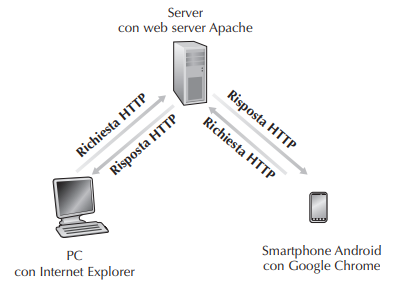
\includegraphics[width=8cm]{images/richiesta-http.PNG}
    \caption{Comportamento richiesta-risposta di HTTP}
    \label{fig:richiesta-http}
\end{figure}

HTTP utilizza TCP (anziché UDP) come protocollo di trasporto. Il client HTTP per prima cosa determina l'URL ed estrae host e filename in modo da iniziare una connessione TCP con il server. Una volta stabilita, il client invia richieste e riceve risposte HTTP, analogamente il server riceve richieste e invia messaggi di risposta.

\subsection{HTTP con connessioni persistenti e non persistenti}
In molte applicazioni per Internet, client e server comunicano per un lungo periodo di tempo, con il client che inoltra una serie di richieste e il server che risponde a ciascuna di esse. A seconda dell'applicazione e del suo impiego la serie di richieste potrebbe essere effettuata in sequenza, periodicamente a intervalli regolari o in maniera intermittente. Quando tale interazione client-server ha luogo su TCP, gli sviluppatori dell'applicazione devono prendere una decisione importante: ciascuna coppia richiesta/risposta deve essere inviata su una connessione TCP separata o devono essere inviate tutte sulla stessa connessione TCP? Nel primo approccio si dice che l'applicazione usa connessioni non persistenti, mentre nel secondo usa connessioni persistenti.

\subsubsection{Connessioni non persistenti}
\begin{Example}{Connessioni non persistenti}{}
    \textit{Seguiamo passo dopo passo il trasferimento di una pagina web dal server al client nel caso di connessioni non persistenti. Supponiamo che la pagina consista di un file HTML principale e di 10 immagini JPEG, e che tutti gli undici oggetti risiedano sullo stesso server. Ipotizziamo che l'URL del file HTML principale sia} \verb|http://www.someSchool.edu/someDepartment/home.index|.

    \begin{enumerate}
        \item Il processo client HTTP inizializza una connessione TCP con il server \verb|www.someSchool.edu| sulla porta 80, che è la porta di default per HTTP.
        Il server HTTP all'host \verb|www.someSchool.edu| in attesa di una connessione TCP alla porta 80 “accetta” la connessione e avvisa il client.
        \item Il client HTTP trasmette un messaggio di richiesta (con l'URL) nella socket della connessione TCP. Il messaggio indica che il client vuole l'oggetto \verb|someDepartment/home.index|.
        \item Il processo server HTTP riceve il messaggio di richiesta, recupera l'oggetto \verb|/someDepartment/home.index| dalla memoria (centrale o di massa), lo incapsula in un messaggio di risposta HTTP che viene inviato al client attraverso la socket.
        \item Il processo server HTTP comunica a TCP di chiudere la connessione.
        \item Il client HTTP riceve il messaggio di risposta. La connessione TCP termina. Il messaggio indica che l'oggetto incapsulato è un file HTML. Il client estrae il file dal messaggio di risposta, esamina il file HTML e trova i riferimenti ai 10 oggetti JPEG.
        \item Vengono quindi ripetuti i primi cinque passi per ciascuno degli oggetti JPEG referenziati.
    \end{enumerate}
\end{Example}

I passi appena riportati illustrano l'utilizzo di connessioni non persistenti, in cui ogni connessione TCP viene chiusa dopo l'invio dell'oggetto da parte del server: vale a dire che ciascuna trasporta soltanto un messaggio di richiesta e un messaggio di risposta. Pertanto, in questo esempio, quando l'utente richiede una pagina web, vengono generate 11 connessioni TCP. 

Prima di procedere facciamo un calcolo approssimativo per stimare l'intervallo di tempo che intercorre tra la richiesta di un file HTML da parte del client e il momento in cui l'intero file viene ricevuto dal client. A questo scopo, definiamo il round-trip time (RTT), che rappresenta il tempo impiegato da un piccolo pacchetto per viaggiare dal client al server e poi tornare al client. RTT include i ritardi di propagazione, di accodamento nei router e nei commutatori intermedi nonché di elaborazione del pacchetto.

Consideriamo ora che cosa succede quando un utente fa click con il mouse su un collegamento ipertestuale. Questa azione fa sì che il browser inizializzi una connessione TCP con il web server. Ciò comporta un handshake (letteralmente, “stretta di mano”) a tre vie (three-way handshake): il client invia un piccolo segmento TCP al server, quest'ultimo manda una conferma per mezzo di un piccolo segmento TCP. Infine, il client dà anch'esso una conferma di ritorno al server. Le prime due parti dell'handshake a tre vie richiedono un RTT. Dopo il loro completamento, il client invia un messaggio di richiesta HTTP combinato con la terza parte dell'handshake. Quando il messaggio di richiesta arriva al server, quest'ultimo inoltra il file HTML sulla connessione TCP. La richiesta-risposta HTTP consuma un altro RTT. Pertanto, il tempo di risposta totale è, approssimativamente, di due RTT, più il tempo di trasmissione da parte del server del file HTML.

\begin{figure}[ht]
    \centering
    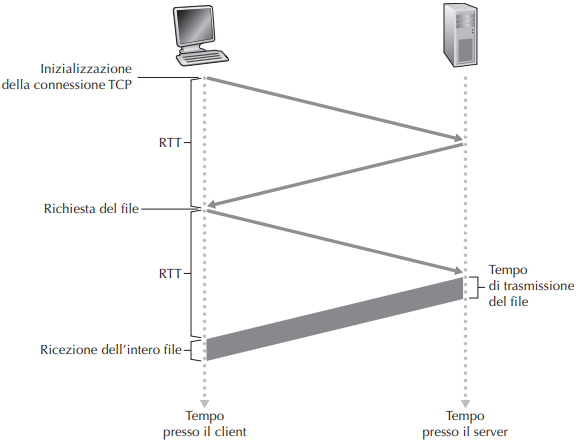
\includegraphics[width=8cm]{images/tempo-html.PNG}
    \caption{Calcolo approssimato del tempo necessario per richiedere e ricevere un file HTML}
    \label{fig:tempo-html}
\end{figure}

\subsubsection{Connessioni persistenti}
Le connessioni non persistenti presentano alcuni limiti: il primo è che per ogni oggetto richiesto occorre stabilire e mantenere una nuova connessione. Per ciascuna di queste connessioni si devono allocare buffer e mantenere variabili TCP sia nel client sia nel server. Ciò pone un grave onere sul web server, che può dover servire contemporaneamente richieste provenienti da centinaia di diversi client. In secondo luogo, come abbiamo appena descritto, ciascun oggetto subisce un ritardo di consegna di due RTT, uno per stabilire la connessione TCP e uno per richiedere e ricevere un oggetto.

Con HTTP nelle connessioni persistenti il server lascia la connessione TCP aperta dopo l'invio di una risposta, per cui le richieste e le risposte successive tra gli stessi client e server possono essere trasmesse sulla stessa connessione. In particolare, non solo il server può inviare un'intera pagina web (nell'esempio, il file HTML principale e le 10 immagini) su una sola connessione TCP permanente, ma può anche spedire allo stesso client più pagine web, in questo modo è necessario solo un solo RTT di connessione per tutti gli oggetti referenziati (+ un RTT per ogni oggetto ricevuto dal server). In generale, il server HTTP chiude la connessione quando essa rimane inattiva per un dato lasso di tempo.

\subsection{Formato dei messaggi HTTP}
Le specifiche HTTP includono la definizione dei due formati dei messaggi HTTP, di richiesta e di risposta.

\subsubsection{Messaggio di richiesta}
\begin{Example}{Messaggio di richiesta HTTP}{}
    \textit{Ecco un tipico messaggio di richiesta HTTP:}
    \begin{lstlisting}
    GET /somedir/page.html HTTP/1.1
    Host: www.someschool.edu
    Connection: close
    User-agent: Mozilla/5.0
    Accept-language: fr
    
    \end{lstlisting}

Notiamo innanzitutto che il messaggio è scritto in testo ASCII, in modo che l'utente sia in grado di leggerlo. Inoltre, notiamo che consiste di cinque righe, ciascuna seguita da un carattere di ritorno a capo (carriage return) e un carattere di nuova linea (line feed). L'ultima riga è seguita da una coppia di caratteri di ritorno a capo e nuova linea aggiuntivi. 

La prima riga è detta riga di richiesta (request line) e quelle successive righe di intestazione (header lines). La riga di richiesta presenta tre campi: il campo metodo, il campo URL e il campo versione di HTTP. Il campo metodo può assumere diversi valori, tra cui \verb|GET|, \verb|POST|, \verb|HEAD|, \verb|PUT| e \verb|DELETE|. Il browser, che implementa la versione \verb|HTTP/1.1|, sta richiedendo l'oggetto \verb|/somedir/page.html|.

La riga \verb|Host: www.someschool.edu| specifica l'host su cui risiede l'oggetto. Includendo la linea di intestazione \verb|Connection: close|, il browser sta comunicando al server che non si deve occupare di connessioni persistenti, ma vuole che questi chiuda la connessione dopo aver inviato l'oggetto richiesto. La riga di intestazione \verb|User-agent:| specifica il tipo di browser che sta effettuando la richiesta al server, in questo caso \verb|Mozilla/5.0|, un browser Firefox. Infine, \verb|Acceptlanguage:| indica che l'utente preferisce ricevere una versione in francese dell'oggetto se disponibile; altrimenti, il server dovrebbe inviare la versione di default.
\end{Example}

A questo punto concentriamoci sul formato generale di un messaggio di richiesta.

\begin{figure}[ht]
    \centering
    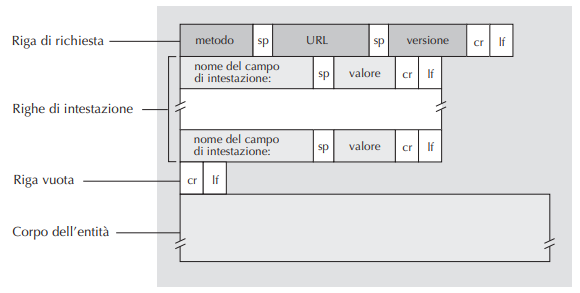
\includegraphics[width=9cm]{images/formato-richiesta.PNG}
    \caption{Formato generale dei messaggi di richiesta di HTTP}
    \label{fig:formato-richiesta}
\end{figure}

Abbiamo visto che i tipi di metodi della riga di richiesta sono: \verb|GET|, \verb|POST|, \verb|HEAD|, \verb|PUT| e \verb|DELETE|.
\begin{itemize}
    \item Il metodo \verb|GET| è usato quando il client vuole scaricare un documento dal server. Il documento richiesto è specificato nell'URL. Il server normalmente risponde con il documento richiesto nel corpo del messaggio di risposta.
    \item Il metodo \verb|POST| è usato per fornire input al server (contenuto dei campi di un form) e, l'input arriva al server nel corpo dell'entità. In realtà le richieste generate con il form non usano necessariamente il metodo \verb|POST|. Anzi, i form HTML usano spesso il metodo \verb|GET| e includono i dati immessi (nei campi del form) nell'URL richiesto. Per esempio, se un form impiega il metodo \verb|GET| e presenta due campi, e se i dati immessi sono scimmie e banane, allora l'URL avrà la struttura: \verb|www.somesite.com/animalsearch?scimmie&banane|. 
    \item Il metodo \verb|HEAD| è simile a \verb|GET|, è usato quando il client non vuole scaricare il documento ma solo alcune informazioni sul documento (come ad esempio la data dell'ultima modifica). Nella risposta il server non inserisce il documento ma solo degli header informativi.
    \item Il metodo \verb|PUT| è utilizzato per memorizzare un documento nel server. Il documento viene fornito nel corpo del messaggio e la posizione di memorizzazione nell'URL. Il metodo \verb|PUT| viene anche utilizzato dalle applicazioni che richiedono di inviare oggetti ai web server. 
    \item Il metodo \verb|DELETE| consente la cancellazione di un oggetto su un server.
\end{itemize}

\subsubsection{Messaggio di risposta}
\begin{Example}{Messaggio di risposta HTTP}{}
    \textit{Presentiamo ora un tipico messaggio di risposta HTTP che potrebbe rappresentare la risposta al messaggio di richiesta dell'esempio precedente.}
    \begin{lstlisting}
    HTTP/1.1 200 OK
    Connection: close
    Date: Thu, 18 Aug 2015 15:44:04 GMT
    Server: Apache/2.2.3 (CentOS)
    Last-Modified: Tue, 18 Aug 2015 15:11:03 GMT
    Content-Length: 6821
    Content-Type: text/html
    (data data data data data ...)
    \end{lstlisting}
    Osserviamo tre sezioni: una riga di stato iniziale, sei righe di intestazione e il corpo. Quest'ultimo è il fulcro del messaggio: contiene l'oggetto richiesto (rappresentato da: \verb|data data data data data ...|). 
    
    La riga di stato presenta tre campi: la versione del protocollo, un codice di stato e un corrispettivo messaggio di stato. In questo esempio, la riga di stato indica che il server sta usando \verb|HTTP/1.1| e che tutto va bene (ossia che il server ha trovato e sta inviando l'oggetto richiesto).
    
    Il server utilizza la riga di intestazione \verb|Connection: close| per comunicare al client che ha intenzione di chiudere la connessione TCP dopo l'invio del messaggio. La riga \verb|Date:| indica l'ora e la data di creazione e invio, da parte del server, della risposta HTTP. Si noti che non si tratta dell'istante in cui l'oggetto è stato creato o modificato per l'ultima volta, ma del momento in cui il server recupera l'oggetto dal proprio file system, lo inserisce nel messaggio di risposta e invia il messaggio. La riga \verb|Server:| indica che il messaggio è stato generato da un web server Apache. La riga \verb|Last-Modified:| indica l'istante e la data il cui l'oggetto è stato creato o modificato per l'ultima volta. La riga di intestazione \verb|ContentLength:| contiene il numero di byte dell'oggetto inviato. La riga \verb|Content-Type:| indica che l'oggetto nel corpo è testo HTML.
\end{Example}

Il codice di stato e l'espressione associata indicano il risultato della richiesta. Tra i più comuni codici di stato e relative espressioni troviamo:
\begin{itemize}
    \item \verb|200 OK|: la richiesta ha avuto successo e in risposta si invia l'informazione.
    \item \verb|301 Moved Permanently|: l'oggetto richiesto è stato trasferito in modo permanente; il nuovo URL è specificato nell'intestazione \verb|Location:| del messaggio di risposta.
    \item \verb|400 Bad Request|: si tratta di un codice di errore generico che indica che la richiesta non è stata compresa dal server.
    \item \verb|404 Not Found|: il documento richiesto non esiste sul server.
    \item \verb|505 HTTP Version Not Supported|: il server non dispone della versione di protocollo HTTP richiesta.
\end{itemize}

\begin{Example}{Esempio GET}{}
    \textit{In questo esempio il client preleva un documento dal percorso} \verb|/usr/bin/image1|.

    \begin{minipage}{\textwidth}
        \centering
        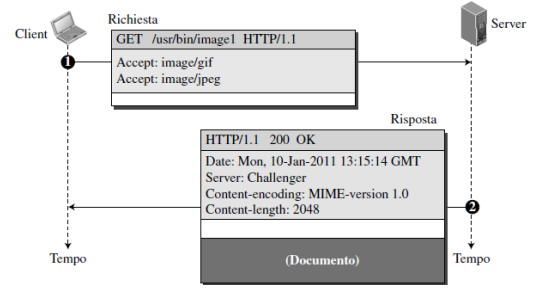
\includegraphics[width=0.6\linewidth]{images/metodo-get.PNG}
        %\captionof{figure}{Esempio}
    \end{minipage}
    
    La riga di richiesta contiene il metodo \verb|GET|, l'URL e la versione \verb|(1.1)| del protocollo HTTP. L'intestazione è costituita da due righe in cui si specifica che il client accetta immagini nei formati \verb|GIF| e \verb|JPEG|. Il messaggio di richiesta non ha corpo. 
    
    Il messaggio di risposta contiene la riga di stato e quattro righe di intestazione che contengono la data, il server, il metodo di codifica del contenuto e la lunghezza del documento. Il corpo del messaggio segue l'intestazione.
\end{Example}

\begin{Example}{Esempio PUT}{}
    \textit{In questo esempio il client spedisce ai server una pagina Web da pubblicare.}

    \begin{minipage}{\textwidth}
        \centering
        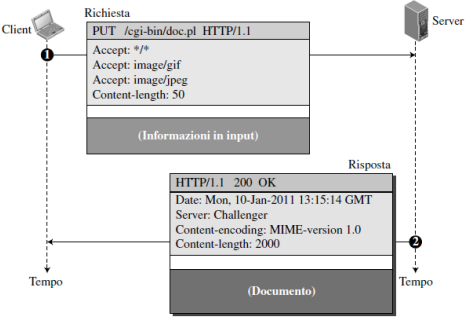
\includegraphics[width=0.6\linewidth]{images/metodo-put.PNG}
        %\captionof{figure}{Esempio}
    \end{minipage}
    
    La riga di richiesta contiene il metodo \verb|PUT|, l'URL e la versione \verb|(1.1)| del protocollo HTTP. L'intestazione è costituita da quattro righe d'intestazione. Il corpo del messaggio di richiesta contiene la pagina Web inviata.
    
    Il messaggio di risposta contiene la riga di stato e quattro righe di intestazione. Il documento creato è incluso nel corpo del messaggio di risposta.
\end{Example}

\subsection{Cookie}
Il Web è stato inizialmente progettato come ambiente "senza stato" (stateless): il server risponde alle richieste inviate dal client senza mantenere alcuna traccia del contesto, senza memorizzare alcuna informazione relativa alla sequenza di richieste inviate dal client, che sono quindi totalmente isolate. Questa modalità è perfettamente in linea con gli obiettivi iniziali del Web: poter ottenere facilmente documenti pubblicamente disponibili. Questo approccio oggi è decisamente inadeguato, visto che il Web ha anche altre funzioni: alcuni siti Web vogliono offrire contenuti personalizzati in base alle preferenze dell'utente; alcuni sisti Web vogliono mantenere il carrello nei siti di commercio elettronico; alcuni siti Web devono limitare l'accesso ai soli utenti registrati.

Tutte queste funzioni richiedono un meccanismo di memorizzazione dello stato o conservazione del contesto: a questo scopo sono stati sviluppati i cookie.

\subsubsection{Interazione utente-server}
La tecnologia dei cookie presenta quattro componenti: 
\begin{enumerate}
    \item una riga di intestazione nel messaggio di risposta HTTP;
    \item una riga di intestazione nel messaggio di richiesta HTTP;
    \item un file cookie mantenuto sul sistema terminale dell'utente e gestito dal browser dell'utente;
    \item un database sul server.
\end{enumerate}

\begin{figure}[ht]
    \centering
    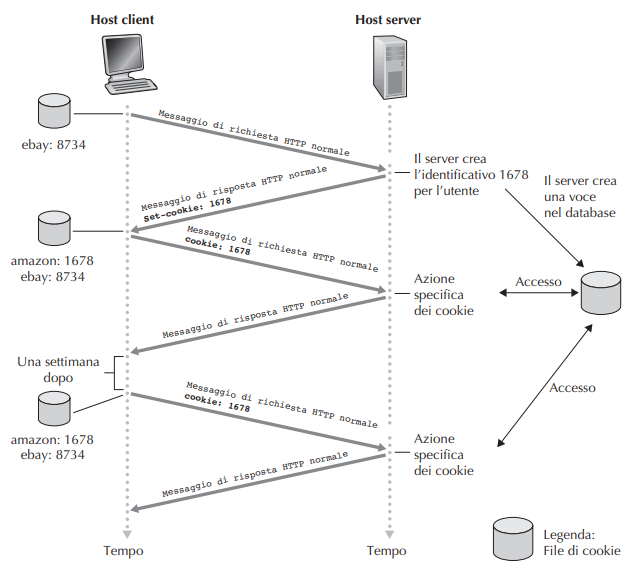
\includegraphics[width=12cm]{images/cookie.PNG}
    \caption{Memorizzazione dello stato dell'utente con i cookie}
    \label{fig:cookie}
\end{figure}

\begin{Example}{Cookie}{}
    \textit{Viene illustrato uno scenario nel quale un negozio elettronico sfrutta opportunamente i cookie.}

    \begin{minipage}{\textwidth}
        \centering
        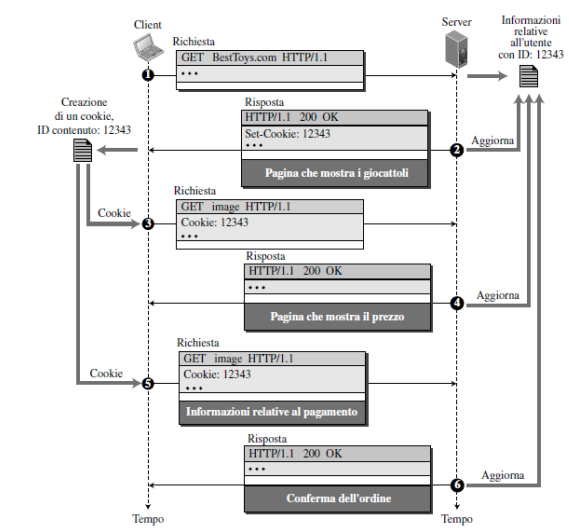
\includegraphics[width=0.7\linewidth]{images/esempio-cookie.PNG}
        %\captionof{figure}{Esempio}
    \end{minipage}

    Si supponga che un cliente desideri comprare un giocattolo da un negozio elettronico chiamato BestToys. \circled{1} Il browser del cliente invia una richiesta al server BestToys. Questo crea per il cliente un carrello della spesa vuoto e gli assegna un identificatore (per esempio 12343). \circled{2} Il server invia quindi un messaggio di risposta che contiene le immagini di tutti i giocattoli disponibili, con un link associato a ciascun giocattolo che consente all'utente di selezionarlo. Questo messaggio di risposta contiene anche la riga di intestazione \verb|Set-Cookie| con valore 12343. Il browser sul computer client visualizza le immagini e memorizza il valore del cookie in un file chiamato BestToys. Il cookie non viene visualizzato al cliente ma solamente memorizzato. \circled{3} Il cliente seleziona ora uno dei giocattoli: il browser invia una richiesta e include l'identificativo 12343 nella riga di intestazione \verb|Cookie|. Sebbene il server stia servendo più clienti contemporaneamente, quando riceve la richiesta e controlla l'intestazione trova il va- lore 12343 come cookie. Il server è quindi in grado di capire che il cliente non è nuovo e cerca quindi il carrello della spesa con identificativo 12343. Il carrello viene aperto per inserirvi il giocattolo scelto. \circled{4} Il server invia ora un'altra risposta al cliente per comunicare il prezzo totale e richiederne il pagamento. \circled{5} Il cliente fornisce le informazioni relative alla propria carta di credito e invia una nuova richiesta, sempre con identificativo 12343 come valore del cookie. \circled{6} Il server che riceve la richiesta riconosce l'identificativo 12343: accetta quindi l'ordine (e il pagamento) e invia una conferma come risposta. Il server archivia le informazioni aggiuntive sul cliente che ha ottenuto durante la transazione. Se il cliente accederà nuovamente al ne- gozio, il browser invierà automaticamente il cookie e il negozio accederà immediatamente a tutte le informazioni archiviate.
\end{Example}

Il cookie inviato al client è un identificatore di sessione (SID). Per evitare che il cookie sia utilizzato da utenti “maligni” l'identificatore è composto da una stringa di numeri. Ad esempio:

\begin{lstlisting}
    == Server -> User Agent ==
    Set-Cookie: SID=31d4d96e407aad42
\end{lstlisting}

Il client ogni volta che manda una richiesta al server fornisce il suo identificatore (cookie): il browser consulta il file cookie, estrae il numero di cookie per il sito che si vuole visitare e lo inserisce nella richiesta http. Ad esempio:
\begin{lstlisting}
    == User Agent -> Server ==
    Cookie: SID=31d4d96e407aad42
\end{lstlisting}

Il server mediante il cookie fornito dal client accede al relativo file e fornisce risposte personalizzate.

Il server chiude una sessione inviando al client una intestazione \verb|Set-Cookie| nel messaggio con
\verb|Max-Age=0|. L'attributo \verb|Max-Age| definisce il tempo di vita in secondi di un cookie. Dopo tot secondi il client dovrebbe rimuovere il cookie. Il valore zero indica che il cookie deve essere rimosso subito.

\subsection{Caching}
Il caching ha come obiettivo migliorare le prestazioni dell'applicazione web. Un modo semplice consiste nel salvare le pagine richieste per riutilizzarle in seguito senza doverle richiedere al server. E' una tecnica efficiente con pagine che vengono visitate molto spesso. Il caching può essere eseguito da Browser o Proxy.

\subsubsection{Browser caching}
Il browser può mantenere una cache delle pagine visitate personalizzabile dall'utente. Esistono vari meccanismi per la gestione della cache locale: l'utente può impostare il numero di giorni dopo i quali i contenuti della cache vengono cancellati; la pagina può essere mantenuta in cache in base alla sua ultima modifica (es. modificata un'ora prima); si possono utilizzare informazioni nei campi intestazione dei messaggi per gestire la cache.

\subsubsection{Web caching: server proxy}
Una web cache, nota anche come proxy server, è un'entità di rete che soddisfa richieste HTTP al posto del web server effettivo. Il proxy ha una propria memoria su disco (una cache) in cui conserva copie di oggetti recentemente richiesti. Il browser di un utente può essere configurato in modo che tutte le richieste HTTP dell'utente vengano innanzitutto dirette al proxy server. Una volta configurato il browser, ogni richiesta di oggetto da parte del browser viene inizialmente diretta al proxy.

\begin{figure}[ht]
    \centering
    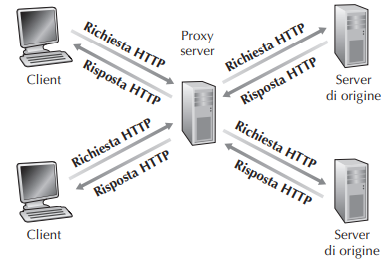
\includegraphics[width=7cm]{images/proxy-server.PNG}
    \caption{Client che richiedono oggetti attraverso un proxy server}
    \label{fig:proxy-server}
\end{figure}

\begin{Example}{Server proxy in una rete locale}{}
    \textit{Si mostra un esempio di impiego di un server proxy in una rete locale, per esempio una rete aziendale o un campus universitario.}

    \begin{minipage}{\textwidth}
        \centering
        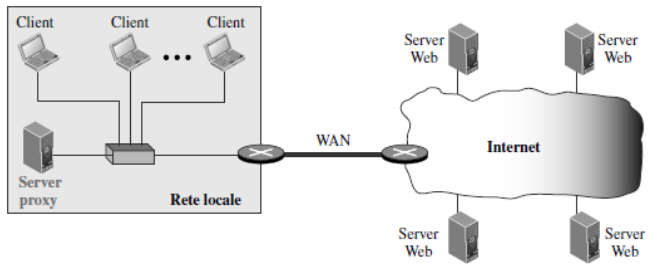
\includegraphics[width=0.7\linewidth]{images/esempio-server-proxy.PNG}
        %\captionof{figure}{Esempio}
    \end{minipage}
    
    Il proxy è installato all'interno della rete locale. Quando il browser di uno dei client genera una richiesta HTTP, questa viene diretta per prima cosa al proxy. Se questi ha già la pagina corrispondente invia la risposta al client. In caso contrario il proxy agisce da client e invia la richiesta al server Web in Internet. Quando la risposta viene restituita, il proxy ne memorizza una copia nella propria memoria cache prima di inviarla al client che l'aveva richiesta.
\end{Example}

Si noti che il proxy è contemporaneamente server e client: quando riceve richieste da un browser e gli invia risposte agisce da server, quando invia richieste e riceve risposte da un server di origine funziona da client.

Generalmente un proxy server è acquistato e installato da un ISP. Per esempio un'università può installare un proxy sulla propria rete e configurare tutti i browser della propria sede per puntare a quel proxy. Oppure un grande ISP (quale ComCast) potrebbe installare uno o più proxy nella propria rete e preconfigurare i browser in modo che vi puntino.

Il web caching si è sviluppato in Internet per due ragioni. Innanzitutto, un proxy può ridurre in modo sostanziale i tempi di risposta alle richieste dei client, in particolare se l'ampiezza di banda che costituisce il collo di bottiglia tra il client e il server di origine è molto inferiore rispetto all'ampiezza di banda minima tra client e proxy. Se esiste una connessione ad alta velocità tra il client e il proxy, come spesso avviene, e se l'oggetto è nella cache, questa sarà in grado di consegnare rapidamente l'oggetto al client. In secondo luogo i proxy possono ridurre sostanzialmente il traffico sul collegamento di accesso a Internet, con il vantaggio di non dover aumentare l'ampiezza di banda frequentemente e ottenere quindi una riduzione dei costi. Inoltre i proxy possono ridurre in modo sostanziale il traffico globale del Web in Internet, migliorando di conseguenza le prestazioni di tutte le applicazioni.

\begin{Example}{Server proxy}{}
    La figura mostra due reti: la rete di un ente e la parte pubblica di Internet.
    
    \begin{wrapfigure}{r}{0.35\textwidth}
        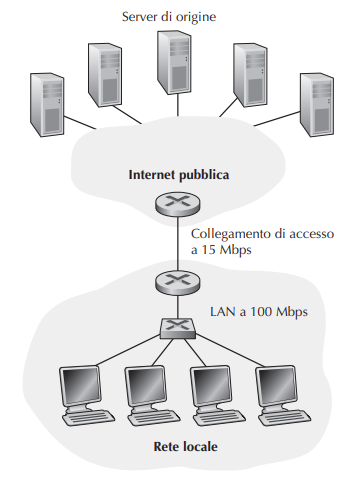
\includegraphics[width=0.33\textwidth]{images/esempio-server-proxy1.PNG}
        %\caption{Birds}
    \end{wrapfigure}
    La rete dell'ente è una LAN ad alta velocità. Un collegamento a 15 Mbps connette un router della prima rete a uno della seconda. Supponiamo che la dimensione media di un oggetto sia 1 Mbit e che i browser dell'ente abbiano una frequenza media di 15 richieste ai server di origine al secondo. Ipotizziamo che i messaggi di richiesta HTTP siano trascurabilmente piccoli e non creino pertanto traffico nelle reti o nel collegamento di accesso (tra i due router). Supponiamo, inoltre, che la quantità di tempo che intercorre da quando il router sul lato Internet del collegamento di accesso inoltra una richiesta HTTP a quando riceve la risposta sia mediamente di due secondi. In modo informale ci riferiamo a questo ultimo ritardo come “ritardo Internet”. Il tempo totale di risposta, ossia il tempo che intercorre tra la richiesta da parte del browser di un oggetto fino alla corrispondente ricezione dell'oggetto, è la somma del ritardo sulla rete locale, del ritardo di accesso (ritardo tra i due router) e del ritardo Internet.
    
    L'intensità di traffico sulla rete locale è pari a:
    \begin{equation*}
        (15 richieste/secondo) * (1 Mbit/richiesta) / (100 Mbps) = 0,15
    \end{equation*}
    mentre l'intensità di traffico sul collegamento di accesso (dal router Internet al router dell'ente) vale:
    \begin{equation*}
        (15 richieste/secondo) * (1 Mbit/richiesta) / (15 Mbps) = 1
    \end{equation*}
    Un'intensità di traffico di 0,15 su una rete locale provoca generalmente alcune decine di millisecondi di ritardo che può, quindi, essere trascurato. Tuttavia quando l'intensità di traffico si avvicina a 1 il ritardo su un collegamento diventa notevole e cresce senza limiti. Pertanto il tempo di risposta medio per soddisfare le richieste diventa dell'ordine dei minuti, se non superiore, il che è inaccettabile per gli utenti. Chiaramente occorre fare qualcosa. Una possibilità consiste nell'incremento della banda sul collegamento di accesso a Internet, per esempio da 15 Mbps a 100 Mbps. Ciò abbasserà l'intensità di traffico sul collegamento di accesso fino a 0,15, il che si traduce in ritardi trascurabili tra i due router. In questo caso, il tempo totale di risposta sarà di circa due secondi, ossia il ritardo Internet. Ma questa soluzione implica che l'ente debba aggiornare il proprio collegamento a Internet, il che può risultare costoso. Una soluzione alternativa consiste nell'adozione di un proxy nella rete dell'istituzione. Le percentuali di successo (o hit rate), cioè la frazione di richieste soddisfatte dalla cache, variano in pratica tra 0,2 e 0,7. A scopo esemplificativo, supponiamo che per la nostra istituzione l'hit rate sia 0,4. Dato che i client e il proxy sono collegati alla stessa rete locale ad alta velocità, il 40\% delle richieste verrà soddisfatto dalla cache quasi immediatamente, ossia entro 10 millisecondi. Ciò nondimeno, il restante 60\% delle richieste deve ancora essere soddisfatto dai server di origine. Ma ora solo il 60\% degli oggetti richiesti passa attraverso il collegamento di accesso, e l'intensità di traffico sul collegamento di accesso si riduce da 1,0 a 0,6. In generale, un'intensità di traffico inferiore a 0,8 su un collegamento a 15 Mbps corrisponde a un piccolo ritardo, dell'ordine delle decine di millisecondi. Questo ritardo è trascurabile rispetto ai due secondi di ritardo Internet. Sulla base di queste considerazioni, il ritardo medio è pertanto:
    \begin{equation*}
        0,4 * (0,01 secondi) + 0,6 * (2,01 secondi)
    \end{equation*}
    che è solo leggermente superiore a 1,2 secondi. Questa seconda soluzione fornisce un tempo di risposta perfino inferiore rispetto alla prima e non richiede l'aggiornamento del collegamento dell'istituzione a Internet. Questa deve, ovviamente, acquistare e installare un proxy, una spesa comunque contenuta: molti proxy sono software di pubblico dominio che possono essere eseguiti su PC economici.
\end{Example}

\subsubsection{GET condizionale}
Sebbene il web caching riduca i tempi di risposta percepiti dall'utente, introduce un nuovo problema: la copia di un oggetto che risiede in cache potrebbe essere scaduta. In altre parole, l'oggetto ospitato nel web server potrebbe esser stato modificato rispetto alla copia nel client (sia esso un proxy o un browser). Fortunatamente, HTTP presenta un meccanismo che permette alla cache di verificare se i suoi oggetti sono aggiornati. Questo meccanismo è chiamato GET condizionale (conditional GET).
Un messaggio di richiesta HTTP viene detto messaggio di GET condizionale se: (1) usa il metodo \verb|GET| e (2) include una riga di intestazione \verb|If-modified-since|.

\begin{Example}{GET condizionale}{}
    Per prima cosa un proxy invia un messaggio di richiesta a un web server per conto del browser richiedente: 
    \begin{lstlisting}
    GET /fruit/kiwi.gif HTTP/1.1
    Host: www.exotiquecuisine.com
    \end{lstlisting}
    Poi, il web server invia al proxy un messaggio di risposta con l'oggetto richiesto: 
    \begin{lstlisting}
    HTTP/1.1 200 OK
    Date: Sat, 3 Oct 2015 15:39:29
    Server: Apache/1.3.0 (Unix)
    Last-Modified: Wed, 9 Sep 2015 09:23:24
    Content-Type: image/gif
    (data data data data data ...)
    \end{lstlisting}
    Il proxy inoltra l'oggetto al browser richiedente e pone anche l'oggetto nella cache locale. Va sottolineato che la cache memorizza con l'oggetto anche la data di ultima modifica. Poi, una settimana più tardi, un altro browser richiede lo stesso oggetto attraverso il proxy, e l'oggetto si trova ancora nella cache. Dato che tale oggetto può essere stato modificato nel web server durante la settimana trascorsa, il proxy effettua un controllo di aggiornamento inviando un GET condizionale. Più nello specifico invia:
    \begin{lstlisting}
    GET /fruit/kiwi.gif HTTP/1.1
    Host: www.exotiquecuisine.com
    If-modified-since: Wed, 9 Sep 2015 09:23:24
    \end{lstlisting}
    Si osservi che il valore della riga di intestazione \verb|If-modified-since:| equivale esattamente al valore della riga di intestazione \verb|Last-Modified:| inviata dal server una settimana prima. Questo GET condizionale sta comunicando al server di inviare l'oggetto solo se è stato modificato rispetto alla data specificata. Supponiamo che l'oggetto non sia stato modificato dalle 9:23:24 del 9 settembre 2015. Allora il web server invia un messaggio di risposta al proxy:
    \begin{lstlisting}
    HTTP/1.1 304 Not Modified
    Date: Sat, 10 Oct 2015 15:39:29
    Server: Apache/1.3.0 (Unix)
    (corpo vuoto)
    \end{lstlisting}
    Notiamo che in risposta a un GET condizionale, il web server invia ancora un messaggio di risposta, ma non include l'oggetto richiesto, in quanto ciò implicherebbe solo spreco di banda e incrementerebbe il tempo di risposta percepito dall'utente, in particolare se l'oggetto è grande. La riga di stato \verb|304 Not Modified| comunica al proxy che può procedere e inoltrare al browser richiedente la copia dell'oggetto presente in cache.
\end{Example}

\section{DNS (Domain Name System)}
Gli host Internet possono essere identificati in vari modi. I nomi degli host (hostname), ad esempio \verb|www.google.com|, risultano abbastanza appropriati per l'uomo, ma forniscono ben poca informazione sulla loro collocazione all'interno di Internet. Inoltre, dato che questi nomi sono costituiti da un numero variabile di caratteri alfanumerici, sarebbero difficilmente elaborabili dai server. Per tali motivi, gli host vengono identificati anche dai cosiddetti indirizzi IP.

Un indirizzo IP consiste di quattro byte e presenta una rigida struttura gerarchica. Ha una forma del tipo \verb|121.7.106.83|, in cui ogni punto separa uno dei byte espressi con un numero decimale compreso tra 0 e 255. Un indirizzo IP è gerarchico perché, leggendolo da sinistra a destra, otteniamo informazioni sempre più specifiche sulla collocazione dell'host in Internet (ossia sulla sua appartenenza a quale rete all'interno della rete di reti).

\subsection{Servizi forniti da DNS}
Abbiamo appena visto che esistono due modi per identificare gli host: il nome e l'indirizzo IP. Le persone preferiscono il primo, mentre i router prediligono gli indirizzi IP a lunghezza fissa e strutturati in modo gerarchico. Al fine di conciliare i due approcci è necessario un servizio in grado di tradurre i nomi degli host nei loro indirizzi IP. Si tratta del principale compito del domain name system (DNS) di Internet. DNS è un database distribuito implementato in una gerarchia di DNS server e un protocollo a livello di applicazione che consente agli host di interrogare il database. Il protocollo DNS utilizza UDP e la porta 53. DNS viene comunemente utilizzato da altri protocolli a livello di applicazione, tra cui HTTP e SMTP, per tradurre i nomi di host forniti dall'utente in indirizzi IP.

\begin{Example}{Interazione con HTTP}{}
    \textit{Consideriamo che cosa succede quando un browser (ossia un client HTTP) in esecuzione sull'host di un utente richiede l'URL} \verb|www.someschool.edu/index.html|\textit{.}

    L'host dell'utente, per essere in grado di inviare un messaggio di richiesta HTTP al web server \verb|www.someschool.edu|, deve come prima cosa ottenere il suo indirizzo IP. Ciò avviene come segue:
    \begin{enumerate}
        \item La stessa macchina utente esegue il lato client dell'applicazione DNS.
        \item Il browser estrae il nome dell'host, \verb|www.someschool.edu|, dall'URL e lo passa al lato client dell'applicazione DNS.
        \item Il client DNS invia una interrogazione (query) contenente l'hostname a un DNS server.
        \item Il client DNS prima o poi riceve una risposta, che include l'indirizzo IP corrispondente all'hostname.
        \item Una volta ricevuto l'indirizzo IP dal DNS, il browser può dare inizio a una connessione TCP verso il processo server HTTP collegato alla porta 80 di quell'indirizzo IP.
    \end{enumerate}
\end{Example}

Oltre alla traduzione degli hostname in indirizzi IP, DNS mette a disposizione altri
importanti servizi:
\begin{itemize}
    \item \textit{Host aliasing}. Un host dal nome complicato può avere uno o più sinonimi (alias). Per esempio, \verb|relay1.west-coast.enterprise.com| potrebbe avere due sinonimi quali \verb|enterprise.com| e \verb|www.enterprise.com|. In questo caso, si dice che il nome \verb|relay1.west-coast.enterprise.com| è un hostname canonico. I sinonimi, se presenti, sono generalmente più facili da ricordare rispetto ai nomi canonici. Il DNS può essere invocato da un'applicazione per ottenere l'hostname canonico di un sinonimo, così come l'indirizzo IP dell'host.
    \item \textit{Mail server aliasing}. Un'applicazione di posta può invocare il DNS per ottenere il nome canonico di un sinonimo fornito, così come l'indirizzo IP dell'host.
    \item \textit{Distribuzione del carico di rete (load distribution)}. Il DNS viene anche utilizzato per distribuire il carico tra server replicati, per esempio dei web server. I siti con molto traffico vengono replicati su più server, ognuno eseguito su un host diverso con un indirizzo IP differente. Nel caso di web server replicati, va dunque associato a ogni hostname canonico un insieme di indirizzi IP. Il database DNS contiene questo insieme di indirizzi. Quando i client effettuano una richiesta DNS per un nome associato a un insieme di indirizzi, il server risponde con l'intero insieme di indirizzi, ma ne varia l'ordinamento a ogni risposta. Dato che generalmente un client invia il suo messaggio di richiesta HTTP al primo indirizzo IP elencato nell'insieme, la rotazione DNS distribuisce il traffico sui server replicati.
\end{itemize}

\subsection{Panoramica del funzionamento DNS}
Dal punto di vista dell'applicazione nell'host utente, il DNS è una scatola nera che fornisce un servizio di traduzione semplice e diretto. Tuttavia nei fatti la scatola nera è costituita da un gran numero di DNS server distribuiti per il mondo e da un protocollo a livello di applicazione che specifica la comunicazione tra DNS server e host richiedenti.
Un primo approccio potrebbe essere quello di utilizzare un DNS server contenente tutte le corrispondenze. In questo schema centralizzato, i client dirigerebbero semplicemente tutte le richieste al singolo server e quest'ultimo risponderebbe loro direttamente. Sebbene tale semplicità progettuale sia attraente, sarebbe inappropriata per l'attuale Internet, dotata di un vasto e sempre crescente numero di host. 
Tra i problemi legati a uno schema centralizzato ricordiamo i seguenti:
\begin{itemize}
    \item \textit{Un solo punto di fallimento.} Se il DNS server si guasta, ne soffre l'intera Internet.
    \item \textit{Volume di traffico.} Un singolo DNS server dovrebbe gestire tutte le richieste (per tutte le richieste HTTP e i messaggi di posta elettronica generati da centinaia di milioni di host).
    \item \textit{Database centralizzato distante.} Un singolo DNS server non può essere vicino a tutti i client. Se il server si trovasse a New York, le query provenienti dall'Australia dovrebbero viaggiare fino all'altro capo del mondo, magari su collegamenti lenti e congestionati, causando ritardi significativi.
    \item \textit{Manutenzione.} Il singolo DNS server dovrebbe contenere record relativi a tutti gli host di Internet. Non solo tale database centralizzato sarebbe vasto, ma dovrebbe essere aggiornato frequentemente per tener conto di ogni nuovo host.
\end{itemize}

In conclusione, un database centralizzato su un singolo DNS server non è in grado
di adattarsi alla crescita esponenziale della rete (ovvero, non è scalabile). Di conseguenza, il DNS è stato progettato in maniera distribuita e costituisce un magnifico
esempio di come si possa implementare un database distribuito su Internet.

\subsubsection*{Gerarchia server DNS}
Per trattare il problema della scalabilità, il DNS utilizza un grande numero di server, organizzati in maniera gerarchica e distribuiti nel mondo. Nessun DNS server ha le corrispondenze per tutti gli host in Internet, che sono invece distribuite tra tutti i DNS
server. In prima approssimazione, esistono tre classi di DNS server: i root server, i
top-level domain (TLD) server e i server autoritativi, organizzati in una gerarchia.

\begin{figure}[ht]
    \centering
    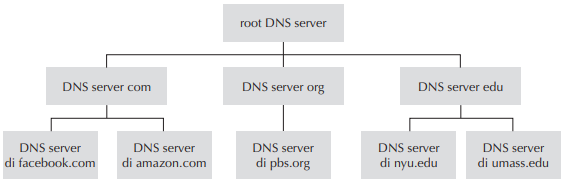
\includegraphics[width=10cm]{images/gerarchia-dns.PNG}
    \caption{Gerarchia di server DNS}
    \label{fig:gerarchia-dns}
\end{figure}

\begin{Example}{Iterazione tra classi DNS}{}
    \textit{Per comprendere l'interazione tra le classi, supponiamo che un client DNS voglia determinare l'indirizzo IP relativo all'hostname} \verb|www.amazon.com|. 
    
    Per fare ciò, il client dapprima contatta uno dei root server, che gli restituisce uno o più indirizzi IP relativi al server TLD per il dominio \verb|com| (detto “dominio di primo livello” o anche “top-level”, in quanto è in cima alla gerarchia). Quindi contatta uno di questi server TLD, che gli restituisce uno o più indirizzi IP del server autoritativo per \verb|amazon.com|. Infine, contatta uno dei server autoritativi per \verb|amazon.com|, che gli restituisce l'indirizzo IP dell'hostname \verb|www.amazon.com|.
\end{Example}

Esaminiamo le tre classi di DNS server:
\begin{itemize}
    \item \textit{Root server.} In Internet esistono 400 root server, dislocati in tutto il mondo. Questi root server sono gestiti da 13 diverse organizzazioni. I root server forniscono gli indirizzi IP dei server TLD.
    \item \textit{Top-level domain (TLD) server.} Questi server si occupano dei domini di primo livello quali \verb|com|, \verb|org|, \verb|net|, \verb|edu| e \verb|gov|, e di tutti i domini di primo livello relativi ai vari paesi, come \verb|uk|, \verb|fr|, \verb|ca| e \verb|jp|. L'azienda Verisign Global Registry Services gestisce i TLD server per il dominio \verb|com| e il Registro.it che ha sede a Pisa all'Istituto di Informatica e Telematica (CNR) gestisce il dominio \verb|it|. I server TLD forniscono gli indirizzi IP dei server autoritativi.
    \item \textit{DNS server autoritativi.} Ogni organizzazione dotata di host pubblicamente accessibili tramite Internet (quali web server e mail server) deve fornire record DNS pubblicamente accessibili che associno i nomi di tali host a indirizzi IP. Il DNS server autoritativo dell'organizzazione ospita questi record. Un'organizzazione può scegliere di implementare il proprio server autoritativo o di pagare un fornitore di servizi per ospitare questi record su un suo server. La maggior parte delle università e delle grandi società implementa e gestisce dei propri server autoritativi primario e secondario (di backup).
\end{itemize}

\begin{figure}[ht]
    \centering
    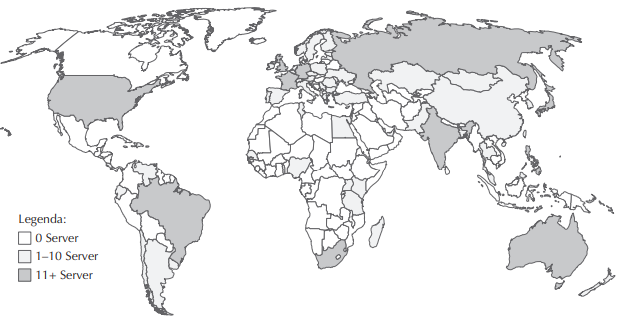
\includegraphics[width=11cm]{images/root-server.PNG}
    \caption{Root DNS server nel mondo}
    \label{fig:root-server}
\end{figure}

Esiste un altro importante tipo di DNS, detto DNS server locale, che non appartiene strettamente alla gerarchia di server, ma che è comunque centrale nell'architettura DNS. Ciascun ISP, come un'università, un dipartimento universitario, un'azienda o un ISP residenziale, ha un DNS server locale (detto anche default name server). Quando un host si connette a un ISP, quest'ultimo gli fornisce un indirizzo IP tratto da uno o più dei suoi DNS server locali. Quando un host effettua una richiesta DNS, la query viene inviata al DNS server locale, che opera da proxy e inoltra la query alla gerarchia dei DNS server.

\begin{Example}{Query DNS iterativa}{}
    \textit{Supponiamo che l'host} \verb|cse.nyu.edu| \textit{voglia l'indirizzo IP di} \verb|gaia.cs.umass.edu|\textit{. Supponiamo, inoltre, che il DNS server locale per} \verb|cse.nyu.edu| \textit{sia} \verb|dns.nyu.edu|\textit{, mentre un server autoritativo per} \verb|gaia.cs.umass.edu| \textit{sia} \verb|dns.umass.edu|. 

     \begin{wrapfigure}{r}{0.35\textwidth}
        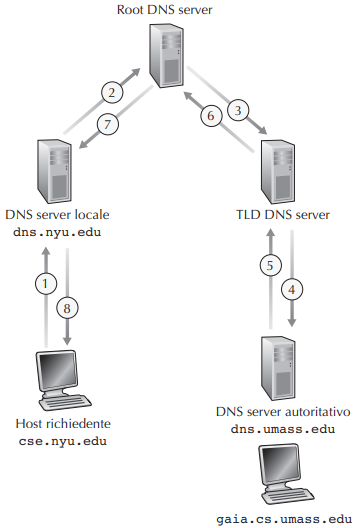
\includegraphics[width=0.33\textwidth]{images/dns-ricorsivo.PNG}
        %\caption{Birds}
    \end{wrapfigure}
    L'host \verb|cse.nyu.edu| dapprima invia un messaggio di richiesta DNS al proprio server locale \verb|dns.nyu.edu|. Il messaggio contiene il nome da tradurre, ossia \verb|gaia.cs.umass.edu|. Il server locale inoltra il messaggio di richiesta a un root server. Quest'ultimo prende nota del suffisso \verb|edu| e restituisce al server locale un elenco di indirizzi IP per i TLD server responsabili di edu. Il server locale rinvia quindi il messaggio di richiesta a uno di questi ultimi. Il TLD server prende nota del suffisso \verb|umass.edu| e risponde con l'indirizzo IP del server autoritativo per l'Università del Massachusetts, ossia \verb|dns.umass.edu|. Infine, il DNS server locale rimanda il messaggio di richiesta direttamente a \verb|dns.umass.edu|, che risponde con l'indirizzo IP di \verb|gaia.cs.umass.edu|.
    
    Si noti che in questo esempio, per ottenere la mappatura di un hostname, sono stati inviati ben otto messaggi DNS: quattro messaggi di richiesta e quattro messaggi di risposta. 
    
    In una query iterativa il server contattato risponde con il nome del server da contattare.
\end{Example}

\begin{Example}{Query DNS ricorsiva}{}
    \begin{wrapfigure}{r}{0.30\textwidth}
        \vspace{-0.6cm}
        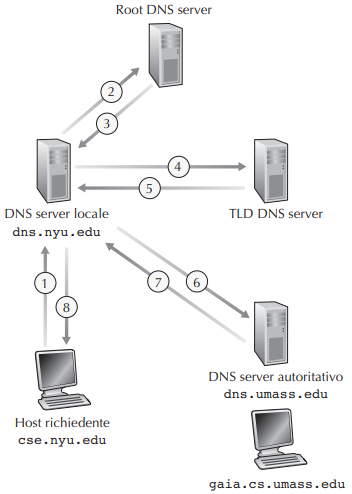
\includegraphics[width=0.28\textwidth]{images/dns-iterativo.PNG}
        %\caption{Birds}
    \end{wrapfigure}
    \textit{Supponiamo ancora che Università del Massachusetts abbia un proprio DNS server, chiamato} \verb|dns.umass.edu|\textit{. Ipotizziamo, inoltre, che ciascun dipartimento dell'università abbia un proprio server, competente per tutti gli host presenti in dipartimento.} 

    In questo caso, quando il DNS server intermedio, \verb|dns.umass.edu|, riceve una richiesta da \verb|dns.nyu.edu| per un host il cui nome termina con \verb|cs.umass.edu|, gli restituisce l'indirizzo IP di \verb|dns.cs.umass.edu|, che rappresenta il server autoritativo per tutti i nomi di host terminanti con \verb|cs.umass.edu|. Il server locale \verb|dns.nyu.edu| invia quindi la richiesta al server autoritativo, che restituisce la corrispondenza desiderata al DNS server locale, il quale a sua volta la restituisce all'host richiedente. 
    
    Una query ricorsiva affida il compito di tradurre il nome al server DNS contattato.
\end{Example}

\subsubsection{DNS caching}
Fino a questo momento abbiamo ignorato il DNS caching, una caratteristica di fondamentale importanza. In verità, il DNS sfrutta in modo estensivo il caching per migliorare le prestazioni di ritardo e per ridurre il numero di messaggi DNS che “rimbalzano” su Internet. L'idea alla base del DNS caching è molto semplice. In una concatenazione di richieste, il DNS server che riceve una risposta DNS (contenente,
per esempio, la traduzione da hostname a indirizzo IP), può mettere in cache le informazioni contenute. Se una coppia hostname/indirizzo IP è nella cache di un DNS server e giunge al server un'altra richiesta con lo stesso hostname, il DNS server può fornire l'indirizzo IP desiderato, anche se non è autoritativo per tale indirizzo. Dato che gli host e le associazioni tra nome e indirizzo IP non sono in alcun modo
permanenti, i DNS server invalidano le informazioni in cache dopo un periodo di tempo fissato (in genere di 2 giorni).  Un DNS server locale può, inoltre, memorizzare in cache gli indirizzi IP dei TLD server, consentendogli di aggirare i root server nella catena di richieste (e ciò avviene di frequente).

\subsection{Record e messaggi DNS}
I server che implementano il database distribuito di DNS memorizzano i cosiddetti record di risorsa (RR, resource record), tra cui quelli che forniscono le corrispondenze tra nomi e indirizzi. Ogni messaggio di risposta DNS trasporta uno o più record di risorse.

Un record di risorsa contiene i seguenti campi: \verb|(Name, Value, Type, TTL)|. \verb|TTL| è il time to live, ossia il tempo residuo di vita di un record e determina quando una risorsa vada rimossa dalla cache. Il significato di \verb|Name| e \verb|Value| dipende da \verb|Type|:
\begin{itemize}
    \item Se \verb|Type=A|, allora \verb|Name| è il nome dell'host e \verb|Value| è il suo indirizzo IP. Pertanto un record di tipo A fornisce la corrispondenza tra hostname standard e indirizzo IP. Per esempio, \texttt{(relay1.bar.foo.com, 145.37.93.126, A)} è un record di tipo A.
    \item Se \verb|Type=NS|, allora \verb|Name| è un dominio (quale \verb|foo.com|) e \verb|Value| è l'hostname del DNS server autoritativo che sa come ottenere gli indirizzi IP degli host nel dominio. Questo record viene usato per instradare le richieste DNS successive alla prima nella concatenazione delle query. Per esempio, \texttt{(foo.com, dns.foo.com, NS)} è un record di tipo NS.
    \item Se \verb|Type=CNAME|, allora \verb|Value| rappresenta il nome canonico dell'host per il sinonimo \verb|Name|. Questo record può fornire agli host richiedenti il nome canonico relativo a un hostname. Per esempio, \texttt{(foo.com, relay1.bar.foo.com, CNAME)} è un record CNAME.
    \item Se \verb|Type=MX|, allora \verb|Value| è il nome canonico di un mail server che ha il sinonimo \verb|Name|. Per esempio, \texttt{(foo.com, mail.bar.foo.com, MX)} è un record MX. Questo tipo di record consente agli hostname dei mail server di avere sinonimi semplici.
\end{itemize}

Un DNS server autoritativo per un certo hostname contiene un record di tipo A per l'hostname. Anche se il server non fosse autoritativo, potrebbe tuttavia contenere un record di tipo A nella propria cache. Se un server non è quello autoritativo per un certo hostname, allora conterrà un record di tipo NS per il dominio che include l'hostname, e conterrà anche un record di tipo A che fornisce l'indirizzo IP del DNS server nel campo \verb|Value| del record NS. 

\begin{Example}{Record DNS}{}
    \textit{Supponiamo che un TLD server non sia competente per l'host} \texttt{corsi.di.uniroma1.it}. 
    
    Allora conterrà un record per un dominio che include l'host \texttt{corsi.di.uniroma1.it}, per esempio \texttt{(umass.edu, dns.umass.edu, NS)}. Il TLD server conterrebbe inoltre un record di tipo A, che indica il DNS server \texttt{dns.uniroma1.it} in un indirizzo IP, per esempio \texttt{(dns.umass.edu, 128.119.40.111, A)}.    
\end{Example}

\subsubsection{Messaggi DNS}
Abbiamo precedentemente fatto riferimento agli unici due tipi di messaggio DNS: le query e i messaggi di risposta che presentano, entrambi, lo stesso formato.

\begin{figure}[ht]
    \centering
    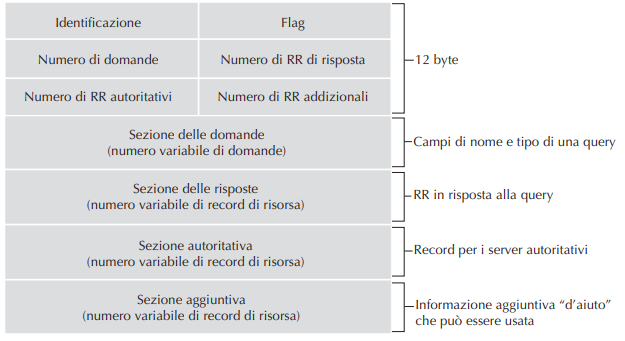
\includegraphics[width=11cm]{images/messaggi-dns.PNG}
    \caption{Formato dei messaggi DNS}
    \label{fig:messaggi-dns}
\end{figure}

La semantica dei campi dei messaggi DNS è la seguente:
\begin{itemize}
    \item I primi 12 byte rappresentano la \textit{sezione di intestazione}, che a sua volta contiene un certo numero di campi. Il primo è un numero di 16 bit che identifica la richiesta. Tale identificatore viene copiato nei messaggi di risposta a una richiesta, consentendo al client di far corrispondere le risposte ricevute con le query inviate. Troviamo poi il campo flag. Il primo di questi, il bit di richiesta/risposta (query/reply), indica se il messaggio è una richiesta (0) o una risposta (1). Un bit viene impostato nei messaggi di risposta quando il DNS server è autoritativo per il nome richiesto. Un ulteriore bit, chiamato di richiesta di ricorsione (recursion-desired flag), viene impostato quando un client (sia esso un host o un DNS server) desidera che il DNS server effettui ricorsione quando non dispone del record. Si imposta un campo da 1 bit di ricorsione disponibile (recursion-available) all'interno di una risposta se il DNS server supporta la ricorsione. Nell'intestazione troviamo anche quattro campi il cui nome comincia con “numero di”, che indicano il numero di occorrenze delle quattro sezioni di tipo dati che seguono l'intestazione.
    \item La \textit{sezione delle domande} contiene informazioni sulle richieste che stanno per essere effettuate. Inoltre, include un campo nome con il nome che sta per essere richiesto, e un campo tipo che indica il tipo della domanda sul nome: per esempio, un indirizzo di host associato a un nome (tipo A) o il server di posta per un nome (tipo MX).
    \item In una risposta proveniente da DNS server, la \textit{sezione delle risposte} contiene i record di risorsa relativi al nome originariamente richiesto. Ricordiamo che in ogni record di risorsa troviamo Type (A, NS, CNAME o MX), Value e TTL. Una risposta può restituire più RR, dato che un hostname può avere più indirizzi IP.
    \item La \textit{sezione autoritativa} contiene i record di altri server autoritativi.
    \item La \textit{sezione aggiuntiva} racchiude altri record utili: per esempio, se il campo di risposta relativo a una richiesta MX contiene un record di risorsa che fornisce l'hostname canonico del server di posta, la sezione aggiuntiva contiene un record di tipo A che fornisce l'indirizzo IP relativo all'hostname canonico del server di posta.
\end{itemize}

\subsubsection{Inserimento di record nel database DNS}
La precedente trattazione si è concentrata su come vengono recuperati i record dal database DNS. A questo punto potreste chiedervi come siano inseriti i record nel database. Vediamolo nel contesto di uno specifico esempio. 

\begin{Example}{Inserimento di record nel database DNS}{}
    \textit{Supponiamo che abbiate appena fondato e avviato una nuova, entusiasmante società chiamata Network Utopia.} 
    
    La prima cosa che sicuramente desiderate fare è registrare il nome di dominio \texttt{networkutopia.com} presso un ente di registrazione (registrar). Un registrar è un'azienda che verifica l'unicità del nome di dominio, lo inserisce nel database DNS e vi richiede una piccola somma di denaro per i propri servizi. Quando registrate il nome di dominio \texttt{networkutopia.com} presso un registrar, dovete fornirgli anche i nomi e gli indirizzi IP dei vostri DNS server autoritativi primario e secondario. Supponiamo che i nomi e gli indirizzi IP siano \texttt{dns1.networkutopia.com}, \texttt{dns2.networkutopia.com}, \texttt{212.2.212.1} e \texttt{212.212.212.2}. Per ciascuno di questi due server autoritativi l'ente si accerterà dell'inserimento di un record di tipo NS e di tipo A nei TLD server relativi al suffisso \verb|com|.  Più nello specifico, per il server autoritativo primario di \texttt{networkutopia.com} il registrar inserirebbe nel sistema DNS i due seguenti record di risorsa: \texttt{(networkutopia.com, dns1.networkutopia.com, NS)} e \texttt{(dns1.networkutopia.com, 212.212.212.1, A)}.

    Dovrete inoltre accertarvi che il record di risorsa di tipo A per il vostro web server \texttt{www.networkutopia.com} e che il record di risorsa di tipo MX per il vostro server di posta \texttt{mail.networkutopia.com} vengano immessi nei vostri DNS server autoritativi. Una volta completati questi passi sarà possibile visitare il vostro sito web e spedire posta elettronica ai dipendenti della vostra società. Concludiamo la nostra trattazione su DNS verificando che questa affermazione sia vera. 

    Supponiamo che Alice, in Australia, voglia visitare la pagina web \texttt{www.networkutopia.com}. Come detto precedentemente, il suo host invierà una richiesta DNS al suo DNS server locale. Quest'ultimo contatterà poi un TLD server per il suffisso \verb|com|. Il DNS server locale dovrà inoltre contattare un root server nel caso in cui l'indirizzo del TLD server responsabile per il suffisso \verb|com| non si trovi in cache. Questo TLD server contiene i record di risorsa di tipo NS e A elencati precedentemente, dato che il registrar li ha inseriti in tutti i TLD server relativi al suffisso \verb|com|. Il TLD server di \verb|com| invia una risposta al server locale di Alice, e la risposta contiene i due record di risorsa. Il server locale invia poi una richiesta DNS a \texttt{212.212.212.1}, cercando il record di tipo A che corrisponde a \texttt{www.networkutopia.com}. Tale record fornisce l'indirizzo IP del web server desiderato, per esempio \texttt{212.212.71.4}, restituito poi dal server locale all'host di Alice. Il browser di Alice può ora inizializzare una connessione TCP verso l'host \texttt{212.212.71.4} e inviare una richiesta HTTP sulla connessione.
\end{Example}

\section{Protocollo FTP}
FTP (File Transfer Protocol) è il protocollo standard offerto da TCP/IP per la copia di file da un host a un altro. Sebbene il trasferimento di un file possa sembrare un'operazione semplice, vi sono, in realtà, numerosi problemi ai quali bisogna prestare attenzione: i due sistemi coinvolti, per esempio, possono adottare convenzioni differenti per la denominazione dei file, oppure gestire in modo differente la struttura delle directory. Problemi di questo tipo vengono risolti in modo semplice ed elegante dal protocollo FTP.

Quando l’utente fornisce il nome dell’host remoto (\verb|ftp NomeHost|), il processo client FTP stabilisce una connessione TCP sulla porta 21 con il processo server FTP. Stabilita la connessione, il client fornisce nome utente e password che vengono inviate sulla connessione TCP come parte dei comandi. Ottenuta l’autorizzazione del server il client può inviare uno o più file memorizzati nel file system locale verso quello remoto (o viceversa).

\begin{figure}[ht]
    \centering
    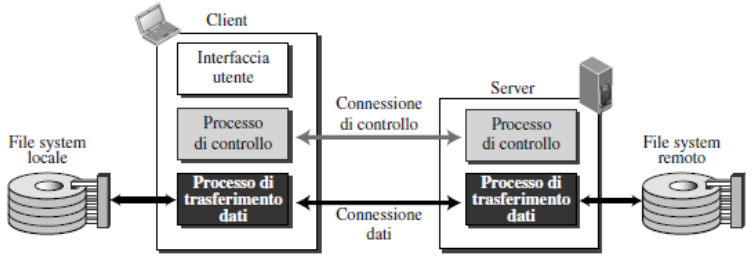
\includegraphics[width=11cm]{images/ftp-client-server.PNG}
    \caption{Protocollo FTP tra client e server}
    \label{fig:ftp-client-server}
\end{figure}

Il client ha tre componenti: interfaccia utente, processo di controllo e processo di trasferimento dati. Il server ha, invece, due sole componenti: processo di controllo e processo di trasferimento dati. La connessione di controllo viene realizzata tra i due processi di controllo e quella per lo scambio dei dati tra i due processi relativi.

La separazione del trasferimento dei dati e dei comandi rende il protocollo FTP piuttosto efficiente: la connessione che si occupa delle informazioni di controllo può usare regole molto semplici, così che lo scambio di informazioni si riduce allo scambio di una riga di comando (o di risposta) per ogni interazione. La connessione che si occupa dello scambio di dati, invece, deve fare uso di regole più complesse a causa della varietà delle informazioni scambiate.

\subsection{Connessione di controllo}
La connessione di controllo (porta 21) viene usata per inviare informazioni di controllo. L’apertura della connessione di controllo viene richiesta dal client al comando \verb|ftp NomeHost| e tutti i comandi eseguiti dall’utente sono trasferiti sulla connessione di controllo.

La comunicazione attraverso la connessione di controllo avviene per mezzo di caratteri con una codifica standard chiamata NVT ASCII, sia per i comandi sia per le risposte. Pur nella sua semplicità questo metodo è perfettamente adeguato perché l'interazione avviene mediante l'invio di un comando o di una risposta alla volta.

Durante questa connessione di controllo i comandi vengono inviati dal client al server e le risposte vengono inviate dal server al client. I comandi sono inviati dal processo di controllo del client FTP sotto forma di caratteri ASCII maiuscoli e possono opzionalmente essere seguiti da un argomento.

Ogni comando FTP genera almeno una risposta; le risposte sono composte da due parti: un numero di tre cifre e un testo. La parte numerica costituisce il codice della risposta, quella di testo contiene i parametri necessari o informazioni supplementari. La prima cifra fornisce lo stato del comando. La seconda cifra definisce l'area alla quale si applica lo stato. La terza cifra fornisce informazioni supplementari. Un esempio di codice di risposta è: \texttt{331 Username OK,
password required}.

\subsection{Connessione dati}
Nella connessione per lo scambio di dati il server usa la porta 20; l'apertura di tale connessione avviene secondo uno schema completamente diverso da quello utilizzato per la connessione di controllo.
\begin{enumerate}
    \item Il client, non il server, effettua un'apertura passiva usando una porta effimera (rimarrà in attesa di connessione); ciò viene fatto dal client perché è tale processo che invierà i comandi per il trasferimento dei file.
    \item Il client invia questo numero di porta al server per mezzo del comando \verb|PORT|.
    \item Il server, ricevuto il numero di porta, effettua un'apertura attiva (aprirà la connessione) usando la porta nota 20 e quella effimera segnalata dal client.
\end{enumerate}

\begin{Example}{Trasferimento di file}{}
    \textit{Viene illustrato un esempio d'uso di FTP per trasferire un file dal server al client.}
    
    \begin{minipage}{\textwidth}
        \centering
        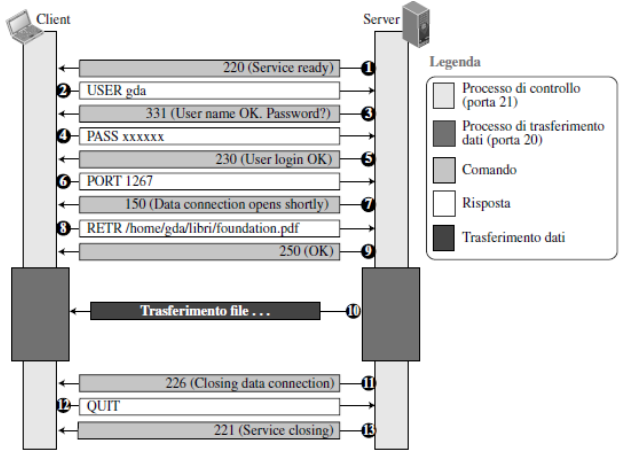
\includegraphics[width=0.7\linewidth]{images/trasferimento-file.PNG}
        %\captionof{figure}{Esempio}
    \end{minipage}
    
     La connessione di controllo rimane sempre aperta, la connessione dati viene invece aperta per il trasferimento del file. Appena completato il trasferimento, il processo di controllo server chiude la connessione dati. Dato che il processo di controllo client non ha altri file da trasferire, invia il comando \verb|QUIT| che fa chiudere la connessione di controllo.
\end{Example}

\section{Posta elettronica}
La posta elettronica (o e-mail) consente agli utenti di scambiarsi messaggi. La natura di questa applicazione è tuttavia differente da altre applicazioni trattate fino a questo momento. Per prima cosa la posta elettronica è considerata una transazione unidirezionale. Quando Gaia invia una e-mail a Gabriele, la risposta non è obbligatoria: Gabriele può decidere di rispondere oppure di non rispondere. Se risponde, si tratta comunque di un'altra transazione unidirezionale. Secondariamente non è ragionevole per Gabriele eseguire un programma server e attendere fino a quando qualcuno gli invia una e-mail. Gabriele potrebbe spegnere il computer quando non lo utilizza. Questo implica che l'idea di programmazione client/server deve essere realizzata in qualche altro modo, ad esempio utilizzando dei computer intermedi (styver).

\subsection{Architettura della posta elettronica}
Abitualmente il mittente e il destinatario della posta elettronica sono collegati via LAN o WAN a due server di posta. L'amministratore ha creato una mailbox (casella di posta) per ogni utente dove memorizzare i messaggi ricevuti. Una mailbox non è altro che una porzione di spazio sulla memoria di massa del server, sotto forma di un file (o di una directory) con opportune restrizioni di accesso per far sì che solamente il proprietario possa accedere. Inoltre, l'amministratore ha creato anche una coda (spesso chiamata spool) dove memorizzare i messaggi in attesa di essere inviati.

\begin{Example}{Invio di una e-mail}{}
    \textit{Il semplice invio di una e-mail da Gaia a Gabriele richiede nove passi.}
    
    Gaia e Gabriele utilizzano tre agenti differenti: un User Agent (UA) usato per scrivere e inviare un messaggio o leggerlo, un Mail Transfer Agent (MTA) usato per trasferire il messaggio attraverso Internet e un Message Access Agent (MAA) usato per leggere la mail in arrivo. 
    
    \begin{minipage}{\textwidth}
        \centering
        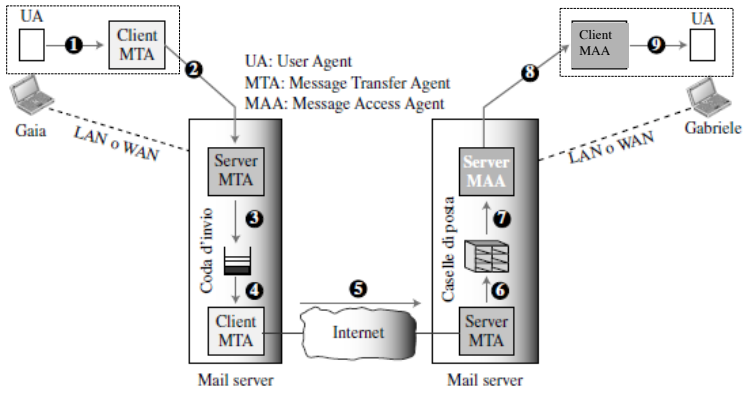
\includegraphics[width=0.8\linewidth]{images/esempio-email.PNG}
        %\captionof{figure}{Esempio}
    \end{minipage}
    
    Gaia, per inviare un messaggio a Gabriele, utilizza un programma UA per preparare il messaggio e inviarlo al proprio server di posta. Quest'ultimo memorizza il messaggio in attesa di essere inviato all'interno di un'apposita coda. Il messaggio, tuttavia, deve essere inviato tramite Internet dal mail server di Gaia al mail server di Gabriele usando un MTA. Sono quindi necessari due MTA in ciascun mail server: uno client e uno server. Analogamente alla maggior parte dei programmi client/server presenti in rete, il server deve essere in esecuzione permanente perché non può sapere quando il client richiederà una connessione. Il client, invece, può essere eseguito dal sistema quando in coda c'è un messaggio in attesa di essere spedito. L'user agent presso il sito di Gabriele gli consente di ricevere e leggere messaggi. Infine Gabriele utilizza un client MAA per ottenere i messaggi da un server MAA in esecuzione sul secondo server.

    Ci sono due aspetti importanti da considerare. Primo, Gabriele è obbligato a passare per il server di posta e non può utilizzare il server MTA direttamente. Per utilizzare il server MTA direttamente, Gabriele dovrebbe mantenerlo sempre in esecuzione perché non può sapere quando arriverà un messaggio.

    Secondo, si noti che Gabriele richiede un'ulteriore coppia di programmi client/server: i programmi per accedere ai messaggi di posta. Il programma client/server MTA, infatti, è un'applicazione di tipo push ("spinta"): il client "spinge" il messaggio al server. Gabriele invece richiede un programma di tipo pull ("tira"): il client deve "tirare" il messaggio dal server.
\end{Example}

Il sistema di posta elettronica richiede due UA, due coppie client/server di MTA e una coppia client/server di MAA.

\begin{figure}[ht]
    \centering
    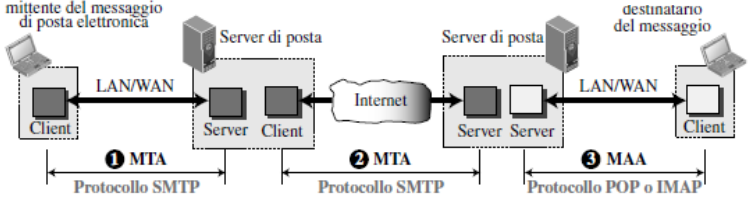
\includegraphics[width=11cm]{images/protocolli-posta.PNG}
    \caption{Protocolli utilizzati nella posta elettronica}
    \label{fig:protocolli-posta}
\end{figure}

\subsection{User agent}
Il primo componente di un sistema di posta elettronica è l'User Agent (UA). Il suo scopo è quello di semplificare all'utente il processo di invio e ricezione dei messaggi. Un user agent è un programma che consente di scrivere, leggere, rispondere e inoltrare i messaggi, ed è in grado inoltre di gestire le mailbox nei computer degli utenti.

Vi sono due tipi di user agent: con interfaccia a riga di comando e con interfaccia grafica (Graphical User Interface, GUI).

L'utente, per inviare una e-mail (tramite l'UA), crea messaggi che sono molto simili alla posta cartacea tradizionale; ogni messaggio di posta elettronica consiste di una sorta di busta (envelope) e del messaggio vero e proprio. La busta contiene solitamente l'indirizzo del destinatario, quello del mittente e altre informazioni. Il messaggio è suddiviso in intestazioni (header) e corpo (body); le intestazioni contengono l'indirizzo del mittente, quello del destinatario, l'argomento del messaggio e alcune altre informazioni, mentre il corpo contiene il messaggio vero e proprio.

\begin{figure}[ht]
    \centering
    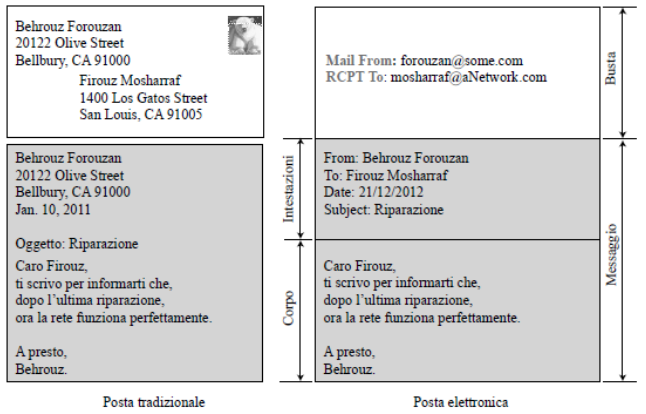
\includegraphics[width=11cm]{images/formato-messaggio.PNG}
    \caption{Formato di un messaggio di posta elettronica}
    \label{fig:formato-messaggio}
\end{figure}

\subsection{Message Transfer Agent: SMTP}
Il protocollo che definisce in modo formale l'interazione tra il client e il server MTA è chiamato SMTP (Simple Mail Transfer Protocol). SMTP è utilizzato in due diverse occasioni: fra il mittente ed il suo server di posta e tra i due server di posta. Quello che fa SMTP è semplicemente definire come deve avvenire l'interazione per mezzo di comandi e risposte.

Il trasferimento di un messaggio di posta elettronica viene realizzato dal protocollo SMTP mediante lo scambio di comandi e risposte tra client e server MTA. I comandi sono inviati da un client MTA a un server MTA, viceversa le risposte. I comandi e le risposte terminano tutti con la medesima coppia di caratteri (ritorno carrello e fine linea).

I comandi vengono inviati dal client al server; il loro formato è composto da una keyword (parla chiave) e uno o più argomenti. Le risposte sono formate da un codice a tre cifre seguito eventualemente da testo.

La consegna di un messaggio avviene in tre fasi distinte: apertura della connessione, trasferimento del messaggio di posta e chiusura della connessione.
\begin{itemize}
    \item \textit{Apertura della connessione.} Il server SMTP dà il via alla fase di apertura della connessione non appena il client effettua la connessione TCP con la porta nota 25.
    \item \textit{Trasferimento del messaggio.} Dopo l'apertura della connessione tra il client e il server SMTP, può essere inviato un singolo messaggio dal mittente a uno o più destinatari.
    \item \textit{Chiusura della connessione.} Il client, una volta trasferito il messaggio, chiude la connessione.
\end{itemize}

\begin{Example}{Trasferimento della posta}{}
    \begin{minipage}[c]{0.55\textwidth}
        Nella parte della figura relativa al trasferimento del messaggio si sono separati i messaggi relativi alla preparazione della busta, dell'intestazione e del corpo. Si noti che la sequenza di passi successivi in questa figura viene ripetuta due volte in ciascun trasferimento di e-mail: la prima dal mittente del messaggio al server di posta locale, la seconda dal server di posta locale al server di posta remoto. Ovviamente, il server di posta locale, una volta ricevuto l'intero messaggio di posta, potrebbe accodarlo per inviarlo al server di posta remoto in un secondo tempo.
    \end{minipage}
    \hfill
    \begin{minipage}[c]{0.44\textwidth}
        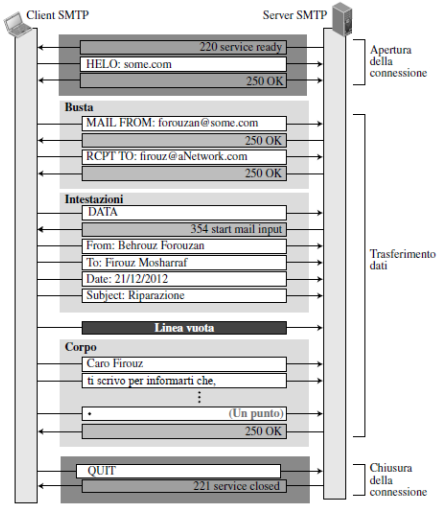
\includegraphics[width=1\textwidth]{images/trasferimento-posta.PNG}
    \end{minipage}
\end{Example}

\subsection{Message Access Agent}
Il primo e il secondo stadio della trasmissione della posta elettronica utilizzano SMTP, che non è invece impiegato nel terzo stadio essendo un protocollo di tipo push: esso "spinge" il messaggio dal client al server. In altri termini, la direzione della maggior parte dei dati (messaggi) è dal client al server. Il terzo stadio richiede invece un protocollo di tipo pull: il client deve "tirare" i messaggi dal server, in questo caso la direzione della maggior parte dei dati è dal server al client. Il terzo stadio utilizza dunque un Message Access Agent.

Attualmente si utilizzano due protocolli per l'accesso ai messaggi: POP3 (Post Office Protocol, versione 3) e IMAP4 (Internet Mail Access Protocol, versione 4).
\begin{itemize}
    \item Il protocollo Post Office Protocol versione 3 (POP3) è molto semplice ma ha funzionalità limitate. Il software client POP3 è installato sul computer del destinatario, mentre il software POP3 server viene installato sul server di posta. L'accesso alla posta avviene quando il client scarica i messaggi (le e-mail) dalla propria casella di posta che si trova sul server. Il client apre una connessione TCP verso il server sulla porta nota 110, quindi invia il proprio nome utente e relativa password per accedere alla casella di posta. A questo punto l'utente può richiedere la lista dei messaggi presenti e prelevarli, uno alla volta.

    Il protocollo POP3 ha due modalità: delete (elimina) e keep (conserva). Nella modalità delete i messaggi sono automaticamente eliminati dalla mailbox dopo il prelievo. Nella modalità keep, invece, i messaggi vengono conservati. La modalità delete viene solitamente utilizzata quando l'utente lavora al proprio computer abituale e può salvare e organizzare la posta ricevuta dopo averla prelevata. La modalità keep è solitamente utilizzata quando l'utente non accede alla posta dalla propria postazione abituale (per esempio da un laptop): in questo caso legge la poste che viene però conservata per l'uso futuro.

    \item Un altro protocollo di accesso alla posta e l'Internet Mail Access Protocol versione 4 (IMAP4). Questo protocollo è simile al POP3 ma ha più funzionalità: è più potente e complesso.
    IMAP4, invece, fornisce varie funzionalità aggiuntive quali: controlla l'intestazione dei messaggi prima del prelievo; ricercare una stringa specifica nei messaggi prima del prelievo; prelevare i messaggi in modo parziale. Una funzionalità particolarmente utile quando vi sono limitazioni di banda; creare, cancellare o rinominare le mailbox sul server di posta; creare una gerarchia di cartelle all'interno della mailbox sul server a scopo di archiviazione.
\end{itemize}

\subsection{Multipurpose Internet Mail Extensions (MIME)}
La posta elettronica ha una struttura molto elementare, ma la sua semplicità comporta che il protocollo possa gestire soltanto messaggi nel formato standard NVT ASCII a 7 bit. Vi sono quindi delle limitazioni; per esempio non possono essere inviati messaggi in lingue che non siano supportate dai caratteri ASCII a 7 bit e non possono essere inviati file binari contenenti audio o video.

Il protocollo MIME (Multipurpose Internet Mail Extensions) è un protocollo supplementare che permette l'invio di messaggi in formati diversi dall'ASCII. Esso agisce lato mittente convertendo tutti i dati in formato non ASCII al formato NVT ASCII e consegnando il risultato al client MTA per l'invio. Il messaggio viene ritrasformato al formato originale presso il destinatario.

In conclusione si può pensare al protocollo MIME come a un insieme di funzioni che si occupano di tradurre dati non ASCII in formato NVT ASCII e viceversa.

\begin{figure}[ht]
    \centering
    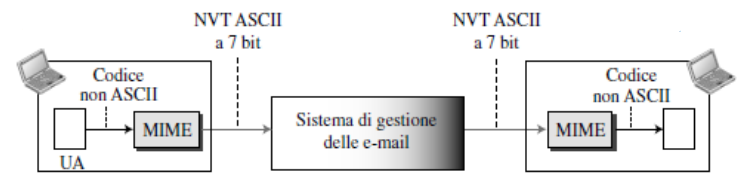
\includegraphics[width=11cm]{images/mime.PNG}
    \caption{Il protocollo MIME}
    \label{fig:mime}
\end{figure}

\subsection{Webmail}
La posta elettronica è un'applicazione talmente comune che vari siti Web offrono questo servizio a chiunque si registri, per esempio Hotmail, Yahoo e Google Mail.

\begin{Example}{Solo il destinatario usa HTTP}{}
    \textit{Gaia, il mittente, utilizza un server di posta tradizionale. Gabriele, il destinatario, ha un account su un server di Webmail.}

    \begin{minipage}{\textwidth}
        \centering
        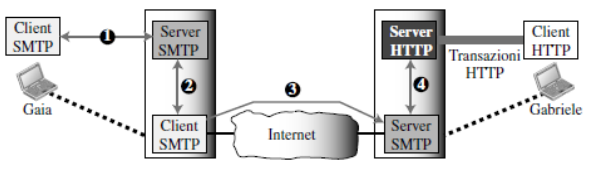
\includegraphics[width=0.6\linewidth]{images/webmail1.PNG}
        %\captionof{figure}{Esempio}
    \end{minipage}
    
    Il trasferimento della posta dall'user agent di Gaia al suo server di posta viene effettuato tramite SMTP. Il trasferimento del messaggio dal server di posta mittente al server di posta destinatario viene nuovamente effettuato via SMTP. Tuttavia il trasferimento del messaggio dal server di destinazione (il server Web) al browser di Gabriele viene effettuo via HTTP. In altri termini, invece di utilizzare POP3 o IMAP si impiega HTTP (o preferibilmente HTTPS). Quando Gabriele vuole prelevare la sua posta, invia un messaggio HTTP di richiesta al sito Web (Hotmail per esempio). Il sito Web invia una form che Gabriele deve completare, che comprende nome utente e password. Se i parametri forniti sono corretti, l'elenco di e-mail viene trasferito dal server Web al browser di Gabriele in formato HTML. Ora Gabriele può scorrere l'elenco e visualizzare le proprie e-mail una alla volta.
\end{Example}

\begin{Example}{Il mittente e il destinatario usano HTTP}{}
    \textit{Sia Gabriele che Gaia usano un server Web, non necessariamente lo stesso.}

    \begin{minipage}{\textwidth}
        \centering
        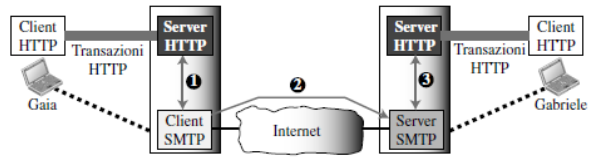
\includegraphics[width=0.6\linewidth]{images/webmail2.PNG}
        %\captionof{figure}{Esempio}
    \end{minipage}
    
    Gaia invia la mail e tutti i dati necessari (per esempio, l'indirizzo di Gabriele) al server Web attraverso HTTP. Il server Web usato da Gaia trasferisce il messaggio al client SMTP e lo invia al server di posta di Gabriele usando il protocollo SMTP. Gabriele riceve il messaggio tramite HTTP.
\end{Example}